\documentclass[a4paper,12pt,titlepage]{article}

% custom paragraph to have line break after using mbox to hack :-/
\newcommand{\myparagraph}[1]{\paragraph{#1}\mbox{}\\}

% import graphicx package so we can import images
\usepackage{graphicx}

\usepackage{framed}

% sensible margins! %
\usepackage[hmargin=3cm,vmargin=2.5cm]{geometry}

\begin{document}

\iffalse
Page 1: Title Page – including the title of the project, the name of the author, the
date, the word count and the statement specified below under report details.
\fi

\begin{titlepage}
    \begin{center}

        { \large Sommelier: A Recommender System}\\[0.4cm]

        { By Peter Chamberlin}

        { \today }

        \vfill

        { 7500 words. }

        { BSc Information Systems and Management Project Report, \\
          Birkbeck College, University of London. }

        \vspace{0.4cm}

        \textit{ This report is the result of my own work except where explicitly stated in the text. The report may be freely copied and distributed provided the source is explicitly acknowledged. }

    \end{center}
\end{titlepage}
\date{\today}




\iffalse
Page 2: Abstract - One page that summarises the report and the main findings or
results.
\fi

\begin{abstract}
    In this project I implement a recommender system as a web service for wine recommendations. As a starting point the I use the wines, authors and ratings data from wine website Decanter.com, and implement a RESTful web API for accessing wine and author information, augmenting the results with recommendations for other wines or authors.
    The system is written in the Python language, using a MySQL database. The API is built using the Flask framework.
    Implementing a primitive collaborative filtering system but finding my source data to be exceptionally sparse for recommendation, I explore and implement imputation techniques using matrix factorization and singular value decomposition in an attempt to boost the system's ability to make good recommendations.
    I find that both matrix factorization and singular value decomposition improve the recommendation quality of the system, but I am unable to satisfactorily test these systems.
\end{abstract}



\iffalse
Page 3: Table of Contents - including page numbers of each chapter heading and
each appendix.
\fi

\tableofcontents

\iffalse 
Chapter 1: Introduction - the topic, the background, why the topic is relevant or of interest to you, what you hoped to achieve, the aims and objectives of the project.  
\fi

\section{Introduction}

\subsection{Online Recommender Systems}

Since their origin in the mid-1990s with systems such as Tapestry \cite{Goldberg92} and GroupLens \cite{Resnick94}, recommender systems have become ubiquitous on the World Wide Web, being employed by some of the worlds largest online businesses as core parts of their offering.

The growth of the Web has given companies the ability to gather unprecedented amounts of data about their users' preferences, both explicitly collected and inferred from their behaviour, while at the same time enabling them to reach users for less cost more often than ever before.

Amazon's system of product recommendations using item-to-item collaborative filtering is regarded as a ``killer feature''\cite{Fortune12}, and is one of the defining features of the Amazon website. The importance of recommendations to Amazon is reflected in their stated mission, ``to delight our customers by allowing them to serendipitously discover great products''\cite{Fortune12}.

Another company which, like Amazon, is synonymous with recommender systems is Netflix, an ``Internet television network'' \cite{NetflixAbout}. In October 2006 Netflix launched ``The Netflix Prize'', a competition with a \$1,000,000 Grand Prize on offer for any team which could beat their own Cinematch recommender system by ``at least 10\%'' accuracy over a fixed set of data \cite{NetflixPrizeRules}. In 2009 the prize was awarded to the BellKor's Pragmatic Chaos team, who had improved on Netflix's own system by 10.06\% \cite{NetflixPrizeCom}. 

As well as online stores using recommender systems to recommend products a user might be interested in, there are systems \ldots

\subsection{Aims and Objectives}

My interest in recommender systems is founded in their variety and ubiquity. It occurred to me that I encounter, and am the subject of, dozens of these systems in my everyday life. Whether it's Twitter or Facebook recommending interesting interesting people or content to me, Amazon recommending me a book or film, or even a supermarket targeting special offers to me, I interact with recommender systems all the time. I am fascinated both by how these systems work theoretically and by how they are implementated in practice. As such the core objective of my project is to implement a recommender system for a web or mobile application.

I have kindly been permitted to freely use data from Decanter.com's wine reviews database \cite{DecanterWine} for my project. The sphere of wine recommendations is particularly interesting; wine is at first glance a narrow subject, but it is a nuanced one. Among oenophiles there is an emphasis on personal taste and a strong tradition of rating and grading. 

In this project I aim to build a recommender system based on Decanter.com's wine database, identifying and overcoming the challenges associated with the implementation of a real-world recommender system.

The most important aspect of any recommender system may be considered to be the quality of its recommendations, and I intend to focus very strongly on recommendation quality. Nevertheless I do not want to overlook the practical implementation of the system. I aim to produce a system satisfactory in both its recommendations and its performance as a web service, with a robust and elegant implementation in code. 

I will not build any kind of graphical interface for the system, but will instead provide a machine readable API, and where necessary batch scripts and command line tools for preparing and manipulating data.

I aim to satisfy several of the most common use cases for wine recommendation, including user-item, item-item and user-user recommendations.

Overall I hope this project will be a strong learning experience for me\ldots



\iffalse
Chapter 2: Literature Review and Context - the setting of the project in the context of other relevant work or theories or results. How this setting influenced the project.
\fi

\section{Literature Review and Context}\label{literature review}

\subsection{Recommender Systems}

Although the term \textit{recommender system} was not coined until 1997 by Resnick and Varian (Resnick and Varian, 1997 \cite{Resnick97}), the Tapestry system of 1992 (Goldberg et al., 1992 \cite{Goldberg92}) is widely recognised as the first of the kind (Su and Khoshoftaar, 2009 \cite{Su09}). The creators of Tapestry coined the term \textit{collaborative filtering} to describe their method of recommendation, which is based on the principle that if two users rate a number of the same items in a similar manner, then it can be assumed that they will rate other new items similarly (Su and Koshgoftaar, 2009\cite{Su09}).

Su and Khoshgoftaar (2009 \cite{Su09}) point out that although collaborative filtering has been widely adopted as a general term to describe systems making recommendations, many such systems do not explicitly collaborate with users or exclusively filter items for recommendation. In fact the term recommender system itself was coined by Resnick and Varian in response to the inadequacy of collaborative filtering for describing the plurality of techniques that were beginning to become associated with it. Recommender system is intentionally a broader term, describing any system that ``assists and augments [the] natural social process'' of recommendation (Resnick and Varian, 1997 \cite{Resnick97}).

In his 2002 survey of the state of the art in recommender systems, Robin Burke presents five categories of recommender (Burke, 2002 \cite{Burke02}). I have reproduced his table of recommendation techniques in Table \ref{table:burke02}. Burke presents five main categories of filtering technique: collaborative, \textit{content-based}, \textit{demographic}, \textit{utility-based} and \textit{knowledge-based} (Burke, 2002 \cite{Burke02}).

\begin{table}[ht]
    \caption{Recommendation Techniques, reproduced from Burke, 2002 \cite{Burke02}}
    \centering
    \begin{tabular}{p{2.5cm} p{3.5cm} p{3.5cm} p{3.5cm}}
        Technique & Backgroud & Input & Process
        \\\hline\hline
        Collaborative & Ratings from \textit{U} of items in \textit{I}. & Ratings from \textit{u} of items in \textit{I}. & Identify users in \textit{U} similar to \textit{u}, and extrapolate from their ratings of \textit{i}. \\
        Content-based & Features of items in \textit{I}. & \textit{u}'s ratings of items in \textit{I}. & Generate a classifier that fits \textit{u}'s rating behaviour and use it on \textit{i}. \\ 
        Demographic & Demographic information about \textit{U} and their ratings of items in \textit{I}. & Demographic information about \textit{u}. & Identify users that are demographically similar to \textit{u}, and extrapolate from their ratings of \textit{i}. \\
        Utility-based & Features of items in \textit{I}. & A utility function over items in \textit{I} that describes \textit{u}'s preferences. & Apply the function to the items and determine \textit{i}'s rank. \\
        Knowledge-based & Features of items in \textit{I}. Knowledge of how these items meet a user's needs. & A description of \textit{u}'s needs or interests. & Infer a match between \textit{i} and \textit{u}'s need. \\
        \\\hline
    \end{tabular}
    \label{table:burke02}
\end{table}

These five kinds of system are classified using three properties: \textit{background data}, \textit{input data} and \textit{process} (Burke, 2002 \cite{Burke02}). Background data is that which exists before and independant of the recommendation, such as previous stated preferences of a group of users \textit{U} for a set of items \textit{I}. Input data is that which is considered by the system when making recommendations, such as the ratings of an individual \textit{u} of items in \textit{I}. Process is the method by which recommendations are arrived at by application of the input data and the background data (Burke, 2002 \cite{Burke02}). These three aspects provide a good lens through which to compare the different approaches.

\subsubsection{Collaborative Filtering}

Collaborative filtering is ``the technique of using peer opinions to predict the interest of others'' (Claypool et al., 1999 \cite{Claypool99}), and uses the ratings of a set of users \textit{U} over a set of items \textit{I} as background data, and the ratings of each individual user \textit{u} of items in \textit{I} as input data. The process of recommendation is to identify similar users to \textit{u} in \textit{U}, and then to infer their preferences for items in \textit{I} based on the preferences of those similar users (Burke, 2002 \cite{Burke02}).

In 2002 Burke described collaborative filtering as the most widely used and mature of these types (Burke, 2002 \cite{Burke02}), citing GroupLens (Resnick, 1994 \cite{Resnick94}) and Tapestry (Goldberg, 1992 \cite{Goldberg92}) as important examples of such systems. From my observations of more recent literature that remains the case. Collaborative filtering is still certainly among the most widely used of these techniques, with Su and Khoshgoftaar describing a large number of collaborative filtering-based systems in their 2009 survey (Su and Koshgoftaar, 2009 \cite{Su09}).

Even in its most basic form there are many potential methods for measuring similarity between users in a collaborative filtering system. The most simple are such distance metrics such as Manhattan distance or Euclidean distance (Segaran, 2007 Ch.2 \cite{Segaran07}). One of the most commonly used and relatively simple measures of similarity is the Pearson correlation coefficient, which is even used in quite advanced systems (Segaran, 2007 Ch.2 \cite{Segaran07}).

There are a number of issues associated with the application of pure collaborative filtering, however, which hamper its application in many instances:

\begin{itemize}
    \item Early rater problem, whereby an item entering the system with no ratings has no chance of being recommended (Claypool et al., 1999 \cite{Claypool99}).
    \item Sparsity problem. Where there is a high ratio of items to ratings it may be difficult to find items which have been rated by enough users to use as the basis for recommendation (Claypool et al., 1999 \cite{Claypool99})(Su and Koshgoftaar, 2009 \cite{Su09}).
    \item Grey sheep, which are users who neither conform nor disagree with any other group in a significant way, making it very difficult to recommend items for them (Claypool et al., 1999 \cite{Claypool99})(Su and Koshgoftaar, 2009 \cite{Su09}).
    \item Synonymy, whereby identical items have different names or entries. In this case the collaborative filtering systems are unable to detect that they are the same item (Su and Koshgoftaar, 2009 \cite{Su09}).
    \item Vulnerability to shilling, where a user may submit a very large number of ratings to manipulate the recommendation of items (Su and Koshgoftaar, 2009 \cite{Su09}).
\end{itemize}

Much of the variation between collaborative filtering techniques described by Su and Khoshgoftaar (2009 \cite{Su09}) can be attributed to efforts by system developers to minimise the impact of one or more of these problems by introducing auxiliary methods.

\subsubsection{Content-based}

In content-based filtering systems the features of items in \textit{I} form the background data, and the user \textit{u}'s ratings serve as the input data. The process of recommendation depends on building a classifier that can predict \textit{u}'s rating behaviour in respect of an item \textit{i} based on \textit{u}'s previous ratings of items in \textit{I} (Burke, 2002 \cite{Burke02}).

Content-based, like collaborative filtering, builds up a long term profile of a user's interests and preferences (Burke, 2002 \cite{Burke02}). Researchers have developed systems which successfully combined content-based and collaborative filtering systems to produce better recommendations. Claypool et al. describe such a system which predicts ratings based on a weighted average of results from each system, with the weighting varying per user in order to achieve optimal results (Claypool et al., 1999 \cite{Claypool99}).

\subsubsection{Demographic}

Demographic recommender systems use demographic information about users \textit{U} and their ratings in \textit{I} as background data, with demographic information about \textit{u} as the input data. The recommendation process depends on matching \textit{u} with other demographically similar users in \textit{U} (Burke, 2002 \cite{Burke02}).

\subsubsection{Utility-based}

Utility-based systems use features of items in \textit{I} as their background data, and depend on a utility function representing \textit{u}'s preferences in order to arrive at recommendations. The process is the application of the function for \textit{u} to the items \textit{I} (Burke, 2002 \cite{Burke02}).

\subsubsection{Knowledge-based}

Knowledge-based systems, like utility-based systems, draw on the features of items in \textit{I} as their background data. As input data they require information about \textit{u}'s needs. The process is to infer a need for one or more items in \textit{I} (Burke, 2002 \cite{Burke02}).

Knowledge-based systems can also benefit from being combined with collaborative filtering systems, in a way that may improve an under-performing knowledge-based system, but without realising pure collaborative filtering's ability to identify niche groups (Burke, 1999 \cite{Burke99b}).

\subsection{Recommending Wines.}

Recommender systems for wines are not a new idea, being typical of the kind of item many systems are designed to recommend. Burke developed the VintageExchange FindMe recommender system in 1999 (Burke, 1999 \cite{Burke99}), and there is at least one patent pending with the WIPO for a wine recommender system as an aid to salespeople or waiting staff (Ward et al., 2012 \cite{WIPO12}).

Burke's FindMe, a knowledge-based recommender system, ``required approximately one person-month of knowledge engineering effort'' (Burke, 1999b \cite{Burke99b}) in order to perform well. Such knowledge-based systems are required to recognise the importance of given product features, and so require a great deal of priming (Burke, 1999b \cite{Burke99b}).

Another wine recommender system is the Tetherless World Wine Agent (TWWA) (Patton, 2010 \cite{Patton10}). The TWWA project is primarily concerned with knowledge representaion and the Semantic Web, presenting a common and collaborative ontology for wine with which users can share wine recommendations across their social networks (TWWA, 2013 \cite{TWWAIndex}). The system does not automatically tailor recommendations to users, although this is stated as a target for future work (TWWA, 2013 \cite{TWWAIndex}).

\subsection{Evaluating Recommender Systems}

Shani and Gunawardana (2011 \cite{Shani11}) describe several approaches to the evaluation of recommender systems, including different experimental settings and a number of different statistical methods. They highlight the different aspects of recommender systems that can be evaluated, including prediction accuracy; how accurately does the system predict ratings or preferences, item-space coverage; what proportion of the items in the system are recommendable, and user-space coverage; the proportion of users or interactions the system can provide recommendations for (Shani and Gunawardana, 2011 \cite{Shani11}).

In terms of prediction accuracy mean absolute error (MAE), and root mean squared error (RMSE) are the most popular measures (Shani and Gunawardana, 2011 \cite{Shani11}), which Su and Khoshgoftaar (2009 \cite{Su09}) call ``predictive accuracy metrics''. 

There is some criticism of accuract metrics applied to recommender systems. McNee, Riedl and Konstan (2006 \cite{McNee06}) cite Amazon.com as a case in point, where on the page for a book by a given author you will find recommendations for other of the same author's books. They argue that this is not interesting for the user, and that there is a need for recommender systems developers to look beyond simply the ratability of systems, concluding, ``It is now time to also study recommenders from a user-centric perspective to make them not only accurate and helpful, but also a pleasure to use'' (McNee et al., 2006 \cite{McNee06}).

\subsection{Web Services and Service Oriented Architecture}

Service oriented architecture (SOA) is an increasingly widely used paradigm in enterprise applications, enabling such benefits as modularity, distribution and reuse of services (Sheikh et al., 2011 \cite{Sheikh11}). SOA systems are loosely coupled, and lend themselves to supporting heterogeneous applications (Benatallah and Nezhad, 2008 \cite{Benatallah08}), such as would be the case for a service providing data for a variety of websites or mobile applications. Web SOAs encompass traditional WS-* web services approaches, such as SOAP and XML, as well as the more recently emerging RESTful (REpresentational State Transfer) approach, which takes advantage of the existing communications protocol of HTTP, and associated protocols such as SSL (Benatallah and Nezhad, 2008 \cite{Benatallah08}). RESTful and WS-* have their benefits and weaknesses, and the choice of either would be dependant on the needs of any given service. 

Pautasso et al. (2008 \cite{Pautasso08}) critically compare WS-* and RESTful services, concluding that although REST is limited by the contraints of the HTTP protocol, its restictive nature and architecture are also a strength, ``choosing REST removes the need for making a series of further architectural decisions related to the various layers of the WS-* stack and makes such complexity appear as superfluous'' (Pautasso et al., 2008 \cite{Pautasso08}).

\subsection{Implications}

There is extensive literature on recommender systems, so much so that it is very difficult to assess the pros and cons of any given approach in respect of my project. One theme that is very strong in recommender systems is that of collaborative filtering, which is central to the majority of systems I have looked at. In many cases collaborative filtering is used in conjunction with other methods that boost or tune the results. For that reason I intend to pursue collaborative filtering in my system, and will incorporate strategies to improve recommendations iteratively.

With regard to the web application component of my system, it seems clear that a RESTful web service would be suitable. My system will have a small number of API endpoints, so I will be able to reap the benefits the simplicity of the RESTful web stack without suffering the difficulties associated with its limited customisability.



\section{Method}\label{method}

\iffalse
the overall approach and rationale.
Why the project was tackled in the chosen way, and why other ways were ruled out.
\fi

\subsection{Methodology}

Given the exploratory nature of this project I elected to take an incremental and iterative approach, developing small parts of the system at any time (increments), and iterating over those parts with improvements as necessity dicated and time allowed. This approach is based on that laid out by Cockburn (2008 \cite{Cockburn08}).

\subsubsection{Phases}

The main phases of development would be:

\begin{enumerate}
    \item Clean up and migrate data
    \item Create initial API app
    \item Connect API with database
    \item Implement routes for API access to wines and authors
    \item Augment API routes for wines and authors with recommendations
    \item Iterate on recommendation methods, evaluating and improving quality
\end{enumerate}

My reason for taking this approach, rather than following a formal development methodology such as the waterfall model, was that my aims and objectives were unbounded, it the sense that there would not be a point at which my system was complete, only a point at which it was minimally complete, followed by a succession of points at which is was improved.

\subsubsection{Minimum Viable Product}

It was clear that I would be doing a large amount of experimental programming, and given my lack of prior experience in the problem domain I felt it inappropriate to attempt to quantify my expectations for the system in terms of detailed requirements. Nevertheless there were very clear minimum objectives for the system, without which it would not be possible to claim any degree of success.

The system should at least:

\begin{itemize}
    \item Provide an HTTP API for accessing wine and user information from the Decanter.com tastings database.
    \item Augment the API results for wines and authors with appropriate recommendations of other similar or interesting wines and author.
    \item Provide API results suitable for machine interpretation by web or mobile applications.
    \item Provide a mechanism by which to evaluate recommendation quality.
\end{itemize}

These requirements in the least should be fulfilled by the system. With this having been done the focus of the project will be on maximising the quality of recommendations.

\subsection{Technologies and Tools}

\subsubsection{Python}

As the main progamming language for my project I chose to use Python. There were several candidate languages, not least Java, but I decided on Python because it has a number of attributes which lent themselves particularly to this project:

\begin{itemize}
    \item Extensive mathematical and scientific libraries, such as numpy \cite{Numpy} and scipy \cite{Scipy}.
    \item Extensive detailed documentation \cite{PythonDocs}.
    \item Widely used in web development, such as by Google and YouTube \cite{PythonQuotes}.
    \item Interactive interpreter, allowing command line interaction and supporting scripting on Unix-like systems \cite{PythonInterpreter}.
\end{itemize}

One deciding factor was that my first enquiry into recommender systems was reading Segaran's code examples in Chapter 2 of Collective Intelligence (2007, Ch.2 \cite{Segaran07}), where the language he uses for his code examples is Python. 

In addition to its suitability for tasks around recommender systems, Python has a solid heritage of web application frameworks, such as Django \cite{DjangoProject} and Flask \cite{Flask}. Django is a fully featured website building framework, and as such carries many features unnecessary for my project, whereas Flask, a ``micro-framework'' \cite{Flask}, appeared to be more lightweight and simple to implement. Therefore I chose to implement my API using Flask \cite{Flask}.

For the most part I considered that my system would suit the stateless, non-persistent nature of a Python web application. The only concern in this regard would be that I would need to recreate objects in memory from scratch with each request rather than persist them as I might using another language, such as using Java with the JPA\cite{JavaJPA}. It was reasonable to suppose that in generating recommendations I would potentially be creating large objects in memory, and that there may be a performance deficit incurred by having to rebuild such object on a per request basis. I resolved that should the lack of persistence prove problematic down the line I would be able to use a persistence mechanism such as Memcached \cite{PythonMemcached} to serve this purpose, and found that there is wide support for such a solution using Python and Flask \cite{FlaskMemcached}.

\subsubsection{MySQL}

Originally I had envisaged a system backed by a PostgreSQL \cite{PostgreSQL} RDBMS, but having received the Decanter.com data as a MySQL \cite{MySQL} database it did not seem, comparing the two systems, that there would be any significant benefit migrating the data to PostgreSQL. Both are widely used in production, and have similar feature sets. For a short time I considered using a NoSQL database such as MongoDB \cite{MongoDB} for my project, but decided against such a solution, recognising that such document-oriented systems are not ideal when joining between tables in the way that I would need to for my wines and tasting notes. It seemed that an RDBMS was ideally suited to the purpose, and there was no reason why that shouldn't be MySQL.

\subsubsection{GitHub}

Given the iterative nature of my development process I envisaged a need to be able to easily version my source code, possibly running several different versions at once, with the ability to revert changes back to any previous state. I also wanted a remote backup of my system in case of problems with my own development computer. In order to do be able to do these things I chose to store my code as a project in GitHub \cite{GitHub}, which is a web service providing Git version control. I chose to use GitHub for my notes and project files also, so that my entire project was stored, versioned and backed up together.



\section{The Sommelier System}\label{design}

\myparagraph{Data Cleanup}

The data source I have used for my project is the wines database belonging to Decanter.com\cite{DecanterCom}. The database contains nearly 40,000 professional ratings and tasting notes for wines from as far back as 1986, featuring vintages as far back as 1917.

The original database is highly inconsistent, displaying a mixture of design approaches and a variable quality of data. This is consistent with the fact that the database has been developed over a long period of time by a number of different developers with varying levels of skill, and that wine journalists making entries into the database have taken a number of idiosyncratic approaches to data entry.

Nevertheless I considered there to be a great deal of useful and interesting information in the database, with it to contain usable ratings and/or tastings for over 33,000 wines.

\begin{figure}[h!]
    \caption{Decanter.com Database}
    \centering
        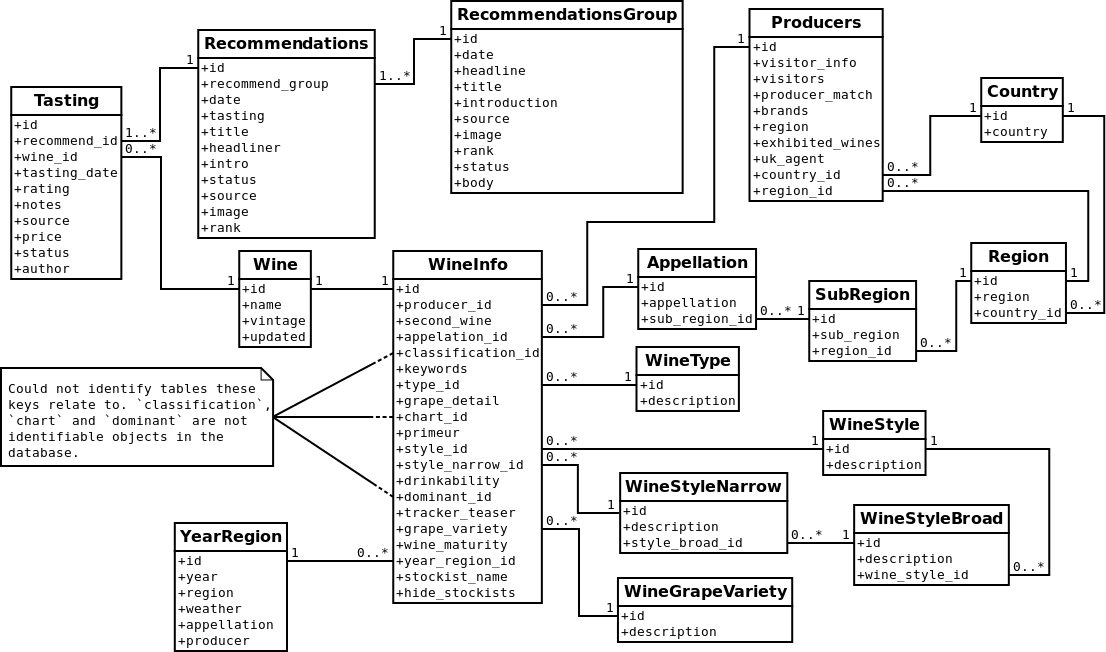
\includegraphics[width=14cm]{DecanterWineDB}
    \label{fig:decanterdb}
\end{figure}

The WineInfo table is a mixture of foreign keys joining to very small tables, such as WineInfo.type\_id joining to WineType.id where WineType is a table with only two attributes. This approach, stiving for a high degree of normalisation, contrasts with the fact that the same table also has the attribute second\_wine, as a string which only holds data in 450 of the 38762 entries in the table.

\myparagraph{Creating The Sommelier Dataset}

\begin{figure}[h!]
    \caption{Sommelier Database}
    \centering
        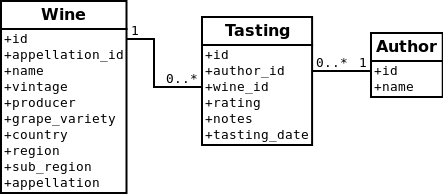
\includegraphics[width=10cm]{SommelierDBSimple}
    \label{fig:sommelierdb}
\end{figure}

For the new Sommelier database, Figure \ref{fig:sommelierdb}, I decided to denormalise [explanation/citation needed!] the wine data. This enables the data to be queried without joins, maximising the simplicity and execution speed of the queries [citation needed]. Denormalization makes data integrity difficult to maintain however, as there are potentially a large number of records to update for any change in a duplicated value. In this case an appellation or sub-region name changing might require thousands of records to be amended. Creating and editing wines is not a requirement of my system though, so for the purposes of this project the wine and tasting data is static and will not be subject to updates. For this reason the duplication of data within the Wine records is not problematic. In a real world setting this would need to be revisited.

Much of the data from the original database was disregarded entirely.

The tables WineStyleNarrow and WineStyleBroad contained generic text descriptions for wine (``rich and creamy'', ``crisp and tangy'' etc.). I initially considered this to have potential for migration into tag data which I could reuse as part of my filtering. Unfortunately less than 6435 of the records in WineInfo had non-null values for their style\_narrow\_id field, and only 3397 of these had corresponding records in the Tasting table. This figure was only around 10\% of the number of wines I expected the Sommelier database to contain so I decided that the WineStyle* tables were probably not worthwhile to migrate.

The WineType table was ignored because no wines corresponded to it; no WineInfo.type\_id record matched any WineType.id.

\myparagraph{The Author Problem}

The biggest shortcoming of the dataset is that the author of a tasting note is often not recorded. The number of wines with notes and known authors is only 1401, with there being 18 named authors on the system. 

Table \ref{table:authors} shows the distribution of tastings amongst authors, only 5 of which have tasted and rated more than 100 wines in the database.

\begin{table}[ht]
\caption{Authors of tasting notes and ratings}
\centering
\begin{tabular}{c c}
\\\hline\hline
Author               & Wines tasted, with notes and rating
\\\hline
Amy Wislocki         &            28 \\
Andrew Jefford       &           105 \\
Beverley Blanning MW &            13 \\
Carolyn Holmes       &             1 \\
Christelle Guibert   &           119 \\
Clive Coates MW      &             6 \\
David Peppercorn     &            44 \\
Gerald D Boyd        &             7 \\
Harriet Waugh        &           250 \\
James Lawther MW     &           226 \\
John Radford         &             2 \\
Josephine Butchart   &            24 \\
Norm Roby            &             4 \\
Rosemary George MW   &             6 \\
Serena Sutcliffe     &            31 \\
Stephen Brook        &            19 \\
Steven Spurrier      &           497 \\
\\\hline
\end{tabular}
\label{table:authors}
\end{table}

In some cases an author's initials or full name are recorded within the text of a tasting note. I decided that extracting and making use of these was impractical given the time constraints of this project.

DESCRIBE DATA SETS BEFORE AND AFTER

THE SOMMELIER DATASET

Having analysed the dataset and conceived an ideal schema, I needed to decide what the criteria to apply when extracting my new dataset from the source data.

Given that the purpose of the dataset is social recommendations, the first decision I made was to discard any wines without both tasting notes and a rating, whether.


\section{Testing and Evaluation}\label{testing}
How well does the system work? Details of testing and evaluation of the system\ldots




\section{Conclusion}\label{conclusions}
Was the project successful?




\section{Review}\label{review}
Review / reflections of the project on a personal level. What has been achieved? What were the problems, and how were they overcome?




\begin{thebibliography}{9}

    \bibitem{Burke99} Burke, R., \emph{The Wasabi Personal Shopper: A Case-Based Recommender System}, 1999. Submitted to the 11th Annual Conference on Innovative Applications of Artificial Intelligence.

    \bibitem{Burke99b} Burke, R., \emph{Integrating Knowledge-Based and Collaborative-Filtering Recommender Systems}, 1999. In: Artificial Intelligence for Electronic Commerce: Papers from the AAAI Workshop (AAAI Technical Report WS-99-0 1), pp.69-72.

    \bibitem{Burke00} Burke, R., \emph{Knowledge-Based Recommender Systems}, Encyclopedia of Library and Information Systems, 2000. Marcel Dekker.

    \bibitem{Burke02} Burke, R., \emph{Hybrid Recommender Systems: Survey and Experiments}, User Modeling and User-Adapted Interaction, Volume 12 Issue 4, November 2002, Pages 331 - 370. Kluwer Academic Publishers: Hingham, MA, USA

    \bibitem{Debnath08} Debnath, Souvik and Ganguly, Niloy and Mitra, Pabitra, \emph{
        Feature weighting in content based recommendation system using social network analysis}, Proceedings of the 17th international conference on World Wide Web, WWW '08, 2008, Beijing, China, Pages 1041 - 1042. ACM: New York, NY, USA,

    \bibitem{Goldberg92} Goldberg, D. Nichols, D., Oki, B. M., and Terry, D., \emph{Using collaborative filtering to weave an information tapestry}, Commun. ACM 35, 12 (Dec. 1992), 61--70.

    \bibitem{Fortune12} Mangalindan, J. P., \emph{Amazon's Recommendation Secret}, July 2012. URL: http://tech.fortune.cnn.com/2012/07/30/amazon-5/

    \bibitem{Patton10} Patton, E., McGuinness, D., \emph{Scaling the Wall: Experiences Adapting a Semantic Web Application to Utilize Social Networks on Mobile Devices}, 2010. In: Proceedings of the WebSci10: Extending the Frontiers of Society On-Line, April 26-27th, 2010, Raleigh, NC: US.

    \bibitem{Resnick94} Resnick, P., Iacovou, N., Sushak, M., Bergstrom, P., Riedl, J., \emph{GroupLens: An open architecture for collaborative filtering of netnews}, 1994 ACM Conference on Computer Supported Collaborative Work, 1994. Association of Computing Machinery, Chapel Hill, NC.

    \bibitem{Resnick97} Resnick, P., Varian, H. R., \emph{Recommender Systems}, 1997. Communications of the ACM, 40 (3), 56-58. Association of Computing Machinery, Chapel Hill, NC.

    \bibitem{TWWAIndex} http://wineagent.tw.rpi.edu/index.php

\iffalse
A. Y. Ng and M. I. Jordan. On discriminative vs generative
classifiers: A comparison of logistic regression and naive
bayes. In Neural Information Processing Systems, pages
841–848, Vancouver, Canada, december 2001. MIT Press.
2
Robles, V.; Larranaga, P.; Menasalvas, E.; Perez, M.S.; Herves, V.; , "Improvement of naive Bayes collaborative filtering using interval estimation," Web Intelligence, 2003. WI 2003. Proceedings. IEEE/WIC International Conference on , vol., no., pp. 168- 174, 13-17 Oct. 2003
doi: 10.1109/WI.2003.1241189
keywords: {Algorithm design and analysis;Clustering algorithms;Collaboration;Collaborative work;Data mining;Filtering algorithms;Probability;Recommender systems;Scalability;Training data; Bayes methods; Web sites; groupware; information filters; learning (artificial intelligence); statistical analysis; Bayesian classifier; UCl repository; Web data; collaborative filtering; ecommerce site; interval estimation; naive Bayes method; recommender system; semi naive Bayes method;}
URL: http://ieeexplore.ieee.org/stamp/stamp.jsp?tp=&arnumber=1241189&isnumber=27823

Xiaoyuan Su; Greiner, R.; Khoshgoftaar, T.M.; Xingquan Zhu; , "Hybrid Collaborative Filtering Algorithms Using a Mixture of Experts," Web Intelligence, IEEE/WIC/ACM International Conference on , vol., no., pp.645-649, 2-5 Nov. 2007
doi: 10.1109/WI.2007.10
keywords: {Clustering algorithms;Collaborative work;Computer science;Filtering algorithms;International collaboration;Motion pictures;Niobium;Predictive models;Recommender systems;USA Councils;information filtering;content-boosted CF;experts mixture;hybrid collaborative filtering algorithms;memory-based algorithms;pure content-based CF algorithms;pure model-based algorithms;sequential mixture CF;}
URL: http://ieeexplore.ieee.org/stamp/stamp.jsp?tp=&arnumber=4427165&isnumber=4427044

Xiaoyuan Su; Taghi M. Khoshgoftaar; , "Collaborative Filtering for Multi-class Data Using Belief Nets Algorithms," Tools with Artificial Intelligence, 2006. ICTAI '06. 18th IEEE International Conference on , vol., no., pp.497-504, Nov. 2006
doi: 10.1109/ICTAI.2006.41
keywords: {Bayesian methods;Collaboration;Collaborative work;Filtering algorithms;Logistics;Predictive models;Recommender systems;Regression tree analysis;Robustness;Scalability;belief networks;data handling;groupware;information filtering;Bayesian belief nets;Pearson correlation-based collaborative filtering;data sparseness;extended logistic regression;multiclass collaborative filtering data;recommender system;tree augmented naive Bayes model;}
URL: http://ieeexplore.ieee.org/stamp/stamp.jsp?tp=&arnumber=4031936&isnumber=4031859



BibTex:

@INPROCEEDINGS{Burke00knowledge-basedrecommender,
author = {Robin Burke},
title = {Knowledge-Based Recommender Systems},
booktitle = {ENCYCLOPEDIA OF LIBRARY AND INFORMATION SYSTEMS},
year = {2000},
pages = {2000},
publisher = {Marcel Dekker}
}

@conference {236,
title = {GroupLens: An open architecture for collaborative filtering of netnews},
booktitle = {1994 ACM Conference on Computer Supported Collaborative Work Conference},
year = {1994},
month = {10/1994},
pages = {175-186},
publisher = {Association of Computing Machinery},
organization = {Association of Computing Machinery},
address = {Chapel Hill, NC},
abstract = {<p class=``abstract''>Collaborative filters help people make choices based on the opinions of other people. GroupLens is a system for collaborative filtering of netnews, to help people find articles they will like in the huge stream of available articles. News reader clients display predicted scores and make it easy for users to rate articles after they read them. Rating servers, called Better Bit Bureaus, gather and disseminate the ratings. The rating servers predict scores based on the heuristic that people who agreed in the past will probably agree again. Users can protect their privacy by entering ratings under pseudonyms, without reducing the effectiveness of the score prediction. The entire architecture is open: alternative software for news clients and Better Bit Bureaus can be developed independently and can interoperate with the components we have developed.</p>},
doi = {http://doi.acm.org/10.1145/192844.192905},
author = {Resnick, P. and Iacovou, N. and Sushak, M. and Bergstrom, P. and J. Riedl}
}


\fi

\end{thebibliography}



\appendix
\scriptsize

\section{Installation} \label{app:installation}

These dependecies should be installed from the command line, having navigated to the project directory.

\begin{verbatim}
# We need pip to be installed to manage python packages
sudo apt-get install python-pip
pip install -U pip

# vitualenv enables us to install modules and packages local to our
# project, so we dont need to expose our system-level python
# installation to incompatible or otherwise obnoxious packages
# that might destabilize our other project, or OS in general
pip install virtualenv
virtualenv flask

# MySQL-python will enable us to query data (very useful!)
# Advice retrieved from http://codeinthehole.com/writing/how-to-set-up-mysql-for-python-on-ubuntu/
# there are some additional dependencies with MySQL-python that need
# to be installed at a system level
sudo apt-get install libmysqlclient-dev python-dev
# Documentation on working with MySQLdb is at: http://mysql-python.sourceforge.net/MySQLdb.html

# now we can install MySQL-python in our virtualenv using a local pip
./flask/bin/pip install MySQL-python

# flask itself is our web framework of choice
./flask/bin/pip install flask

# mock will be useful for unit testing
./flask/bin/pip install mock

# nose will serve as our test runner
# https://nose.readthedocs.org/en/latest/ Source: https://github.com/nose-devs/nose
./flask/bin/pip install nose

# gonna need numpy a lot probably!
# scipy is a pain. The following installation method is courtesy of:
# http://www.scipy.org/Installing_SciPy/Linux#head-d437bf93b9d428c6efeb08575f631ddf398374ea
# This installs rather a lot of stuff :-|
sudo apt-get build-dep python-numpy 
# the following command does a big build and throws all sorts of errors, which are apparently fine to ignore.
sudo apt-get -b source python-numpy 
./flask/bin/pip install scipy 

# install dependencies for python-recsys
flask/bin/pip install csc-pysparse networkx divisi2
# clone python-recsys from Git and set it up in virtualenv
git clone http://github.com/ocelma/python-recsys
cd python-recsys
../flask/bin/python setup.py install

# install matplotlib for graphing test results
# n.b. this is not subsequently installed in the virtualenv, but
# that isnt a problem as the graphing can be done without
# invoking any of our virtualenv
sudo apt-get install python-matplotlib
\end{verbatim}

\section{Source Data} \label{app:data}

\subsection{Migration} \label{app:datamigration}

The notes in this section include the commands that recreate the migration of data from the original Decanter.com wines database to the Sommelier database.

\subsubsection{Convert to UTF-8}

\begin{verbatim}
## Conversion from latin1 to utf8:

Based on advice from: http://en.gentoo-wiki.com/wiki/Convert_latin1_to_UTF-8_in_MySQL

From the Bash shell:
$ mysqldump -uroot -p -hlocalhost --default-character-set=latin1 -c --insert-ignore --skip-set-charset -r wine_dump.sql wine
$ file wine_dump.sql
> wine_dump.sql: Non-ISO extended-ASCII English text, with very long lines
$ iconv -f ISO8859-1 -t UTF-8 wine_dump.sql > wine_dump_utf8.sql
$ sed -i 's/latin1/utf8/g' wine_dump_utf8.sql

Now, from the MySQL command line:
mysql> CREATE DATABASE sommelier CHARACTER SET utf8 COLLATE utf8_general_ci;

And finally, back in the Bash shell:
$ mysql -uroot --max_allowed_packet=16M -p --default-character-set=utf8 sommelier < wine_dump_utf8.sql

\end{verbatim}

\subsubsection{Create Sommelier Tables}

This is the code for creating the new Sommelier database tables. The code is executed on a copy of the original database which has been duplicated with a new name. After creating the new tables, the old tables are deleted and the new tables are renamed to the old names (wine, author, tasting).

\begin{verbatim}
Content for sommelier.wine:

CREATE TABLE `sommelier_wine` (
  `id` int(11) NOT NULL AUTO_INCREMENT,
  `name` varchar(255) NOT NULL DEFAULT '',
  `vintage` int(4) NOT NULL DEFAULT '0',
  `grape_variety` varchar(255) NOT NULL DEFAULT '',
  `producer` varchar(255) NOT NULL DEFAULT '',
  `country` varchar(255) NOT NULL DEFAULT '',
  `region` varchar(255) NOT NULL DEFAULT '',
  `sub_region` varchar(255) NOT NULL DEFAULT '',
  `appellation` varchar(255) NOT NULL DEFAULT '',
  PRIMARY KEY (`id`)
) ENGINE=MyISAM AUTO_INCREMENT=1 DEFAULT CHARSET=utf8;

INSERT INTO sommelier_wine SELECT 
  w.id,
  w.name AS name, 
  w.vintage AS vintage, 
  p.producer_match AS producer, 
  gv.description AS description,
  c.country AS country,
  r.region AS region,
  sr.sub_region AS sub_region,
  a.appellation AS appellation
FROM
  wine w 
JOIN wine_info wi ON w.id = wi.id 
LEFT JOIN producers p ON p.id = wi.producer_id 
LEFT JOIN wine_grape_variety gv ON gv.id = wi.grape_variety 
LEFT JOIN appellation a ON a.id = wi.appellation_id
LEFT JOIN sub_region sr ON sr.id = a.sub_region_id
LEFT JOIN region r ON r.id = sr.region_id
LEFT JOIN country c ON c.id = r.country_id
ORDER BY w.id ASC;

CREATE TABLE `sommelier_author` (
  `id` int(11) NOT NULL AUTO_INCREMENT,
  `name` varchar(255) NOT NULL DEFAULT '',
  PRIMARY KEY (`id`)
) ENGINE=MyISAM AUTO_INCREMENT=1 DEFAULT CHARSET=utf8;

INSERT INTO sommelier_author SELECT DISTINCT
  NULL,
  t.author as name
FROM
  tasting t
WHERE t.author <> '';

CREATE TABLE `sommelier_tasting` (
  `id` int(11) NOT NULL AUTO_INCREMENT,
  `wine_id` int(11) NOT NULL,
  `author_id` int(11) NOT NULL,
  `rating` int(11) NOT NULL,
  `notes` TEXT NOT NULL,
  `tasting_date` datetime NOT NULL DEFAULT '0000-00-00 00:00:00',
  PRIMARY KEY (`id`),
  KEY `wine_idx` (`wine_id`),
  KEY `author_idx` (`author_id`)
) ENGINE=MyISAM AUTO_INCREMENT=1 DEFAULT CHARSET=utf8;

INSERT INTO sommelier_tasting SELECT
  NULL,
  t.wine_id AS wine_id,
  a.id AS author_id,
  t.rating AS rating,
  t.notes AS notes,
  t.tasting_date AS tasting_date
FROM
  tasting t 
JOIN wine w ON w.id = t.wine_id 
JOIN wine_info wi ON w.id = wi.id 
LEFT JOIN sommelier_author a ON t.author = a.name
WHERE t.rating > 0 
  AND t.notes <> '' 
ORDER BY w.id ASC;

Finally, delete all wines without tasting records:

DELETE FROM sommelier_wine WHERE id NOT IN ( SELECT wine_id FROM sommelier_tasting );

DROP TABLE wine;
DROP TABLE tasting;
DROP TABLE author;

RENAME TABLE sommelier_wine TO wine;
RENAME TABLE sommelier_tasting TO tasting;
RENAME TABLE sommelier_author TO author;
\end{verbatim}

\subsection{Sparsity} \label{app:datasparsity}

Sparsity of 94\% calculated by:

Distinct number of known authors in tasting table: 18

Total number of tastings by known authors: 1411

Distinct number of wine ids in tasting table with known author: 1307

Sparsity percentage = $100 - (( 1411 \div ( 1307 \times 18 )) \times 100) $

\subsection{Author Similarity} \label{app:authorsim}

Table data obtained in the Python interactive interpreter by the following commands (see also \ref{app:recommendations}):

\begin{verbatim}
import recommendations
recommendations.getAuthorSimilarities()
\end{verbatim}

\section{API Design}

\subsection{API Routes}

\subsubsection{API Response: Index}\label{app:apiindex}
\begin{verbatim}
{
    ``type'': ``list'',
    ``self'': {
        ``title'': ``Sommelier API'',
        ``link'': ``/''
    },
    ``list'': [
        {
        ``title'': ``All Authors'',
        ``link'': ``/authors/1''
        },
        {
        ``title'': ``All Wines'',
        ``link'': ``/wines/1''
        }
    ]
}
\end{verbatim}

\subsubsection{API Response: Authors}\label{app:apiauthors}
\begin{verbatim}
{
    ``type'': ``list'',
    ``self'': {
        ``title'': ``Authors, Page 1''
        ``link'': ``/authors/1''
    },
    ``list'': [
        /* maximum 50 links per page */
        {
        ``title'': ``Mr. Author'',
        ``link'': ``/author/123''
        },
        {
        ``title'': ``A.N. Other'',
        ``link'': ``/author/234''
        }
    }
}
\end{verbatim}
    
\subsubsection{API Response: Author}\label{app:apiauthor}
\begin{verbatim}
{
    ``type'': ``author'',
    ``self'': {
        ``title'': ``Mr. Author'',
        ``name'': ``Mr. Author'',
        ``tastings'': [
            {
            ``rating'': 5,
            ``notes'': ``Tasting notes about the wine'',
            ``tasting_date'': ``2003-04-01 00:00:00'',
            ``wine'': {
                ``title'': ``Wine Name 1990'',
                ``link'': ``/wine/123''
            }
        ],
        ``link'': ``/author/123''
    },
    ``related_content'': {
        /* maximum of 5 wines */
        ``recommended_wines'': [
            {
            ``title'': ``Chateau du Vin 1996'',
            ``link'': ``/wine/234''
            }
        ],
        /* maximum of 5 other authors */
        ``similar_authors'': [
            {
            ``title'': ``A.N. Other'',
            ``link'': ``/author/234''
            }
        ]
    }
}
\end{verbatim}

\subsubsection{API Response: Wines}\label{app:apiwines}
\begin{verbatim}
{
    ``type'': ``list''
    ``self'': {
        ``title'': ``Wines, Page 1''
        ``link'': ``/wines/1''
    },
    ``list'': [
        /* maximum 50 links per page */
        {
        ``title'': ``Wine Name 1990'',
        ``link'': ``/wine/123''
        },
        {
        ``title'': ``Chateau du Vin 1996'',
        ``link'': ``/wine/234''
        }
    }
}
\end{verbatim}

\subsubsection{API Response: Wine}\label{app:apiwine}

\begin{verbatim}
{
    ``type'': ``wine'',
    ``self'': {
        ``title'': ``Wine Name 1990'',
        ``name'': ``Wine Name'',
        ``vintage'': 1990,
        ``producer'': ``Wine Producer Name'',
        ``grape_variety'': ``Cabernet Sauvignon'',
        ``appellation'': ``Pessac-Leognan'',
        ``country'': ``France'',
        ``region'': ``Bordeaux'',
        ``sub_region'': ``Graves''
        ``tastings'': [
            {
            ``rating'': 5,
            ``notes'': ``Tasting notes about the wine'',
            ``tasting_date'': ``2003-04-01 00:00:00'',
            ``author'': {
                ``title'': ``Mr. Author'',
                ``link'': ``/author/123''
            }
        ],
        ``link'': ``/wine/123''
    },
    ``related_content'': {
        /* maximum of 5 wines */
        ``similar_wines'': [
            {
            ``title'': ``Chateau du Vin 1996'',
            ``link'': ``/wine/2345''
            }
        ]
    }
}
\end{verbatim}

\section{Experimental Code}

\subsection{Code derived from Segaran, 2007} \label{app:recommendations}

This code was copied largely from Segaran's exercises in Ch.2 of Collective Intelligence (2007). I have truncated part of the data fixture for brevity.

I have adapted Segaran's code, implementing new methods to query data from the Sommelier database and apply his methods to that data.

\begin{verbatim}
# a dictionary of critics and their ratings of a small
# set of movies
# copied from Segaran: Collective Intelligence (2006) Ch.2
critics={
    'Lisa Rose': {
        'Lady in the Water': 2.5,
        'Snakes on a Plane': 3.5,
        'Just My Luck': 3.0,
        'Superman Returns': 3.5,
        'You, Me and Dupree': 2.5,
        'The Night Listener': 3.0
    },
#### TRUNCATED ####
    'Toby': {
        'Snakes on a Plane': 4.5,
        'Superman Returns': 4.0,
        'You, Me and Dupree': 1.0
    }
}

# Method copied from Segaran: Collective Intelligence (2006) Ch.2
from math import sqrt
def sim_distance(prefs,person1,person2):
    si={}
    for item in prefs[person1]:
        if item in prefs[person2]:
            si[item]=1
    if len(si)==0: return 0
    sum_of_squares=sum([pow(prefs[person1][item]-prefs[person2][item],2)
    return 1/(1+sum_of_squares)

# This method is equivalent to sim_distance() above, uses scipy's sqeuclidean method
import scipy.spatial
def euclidean_distance(prefs,person1,person2):
    vector1=[]
    vector2=[]
    for item in prefs[person1]:
        if item in prefs[person2]:
            vector1.append(prefs[person1][item])
            vector2.append(prefs[person2][item])
    if len(vector1)==0: return 0
    euclidean_distance=scipy.spatial.distance.sqeuclidean(vector1,vector2)
    return 1 / (1 + euclidean_distance)

# Method copied from Segaran: Collective Intelligence (2006) Ch.2
def sim_pearson(prefs,p1,p2):
    si={}
    for item in prefs[p1]:
        if item in prefs[p2]: si[item]=1
    n=len(si)
    if n==0: return 0
    sum1=sum([prefs[p1][it] for it in si])
    sum2=sum([prefs[p2][it] for it in si])
    sum1Sq=sum([pow(prefs[p1][it],2) for it in si])
    sum2Sq=sum([pow(prefs[p2][it],2) for it in si])
    pSum=sum([prefs[p1][it]*prefs[p2][it] for it in si])
    # calculate Pearson score:
    num=pSum-(sum1*sum2/n)
    den=sqrt((sum1Sq-pow(sum1,2)/n)*(sum2Sq-pow(sum2,2)/n))
    if den==0: return 0
    r=num/den
    return r

# Method copied from Segaran: Collective Intelligence (2006) Ch.2
def topMatches(prefs,person,n=5,similarity=sim_pearson):
    scores=[(similarity(prefs,person,other), other)
            for other in prefs if other!=person]
    scores.sort()
    scores.reverse()
    return scores[0:n]

# Method copied from Segaran: Collective Intelligence (2006) Ch.2
# Gets recommendations for a person by using weighted average
# of every other user's rankings
def getRecommendations(prefs,person,similarity=sim_pearson):
    totals={}
    simSums={}
    for other in prefs:
        if other==person: continue
        sim=similarity(prefs,person,other)
        if sim<=0: continue
        for item in prefs[other]:
            # only score movies 'person' hasn't seen
            if item not in prefs[person] or prefs[person][item]==0:
                # similarity*score
                totals.setdefault(item,0)
                totals[item]+=prefs[other][item]*sim
                # sum of similarities
                simSums.setdefault(item,0)
                simSums[item]+=sim
    rankings=[(total/simSums[item],item) for item,total in totals.items()]
    rankings.sort()
    rankings.reverse()
    return rankings

# Method copied from Segaran: Collective Intelligence (2006) Ch.2
def transformPrefs(prefs):
    result={}
    for person in prefs:
        for item in prefs[person]:
            result.setdefault(item,{})
            result[item][person]=prefs[person][item]
    return result

# Method copied from Segaran: Collective Intelligence (2006) Ch.2
def calculateSimilarItems(prefs,n=10,similarity=sim_distance):
    result={}
    itemPrefs=transformPrefs(prefs)
    c=0
    for item in itemPrefs:
        c+=1
        if c%100==0: print "%d / %d" % (c,len(itemPrefs))
        scores=topMatches(itemPrefs,item,n=n,similarity=sim_distance)
        result[item]=scores
    return result

# Method copied from Segaran: Collective Intelligence (2006) Ch.2
def getRecommendedItems(prefs,itemMatch,user):
    userRatings=prefs[user]
    scores={}
    totalSim={}
    for (item,rating) in userRatings.items():
        for (similarity, item2) in itemMatch[item]:
            if item2 in userRatings: continue
            # Weighted sum of rating times similarity
            scores.setdefault(item2,0)
            scores[item2]+=similarity*rating
            # Sum of all the similarities
            totalSim.setdefault(item2,0)
            totalSim[item2]+=similarity
    # Divide each total score by total weighting to give an average
    rankings=[(score/totalSim[item],item) for item,score in scores.items()]
    rankings.sort()
    rankings.reverse()
    return rankings

# Method copied from Segaran: Collective Intelligence (2006) Ch.2
def loadMovieLens(path='../data/ml-100k'):
    movies={}
    for line in open(path+'/u.item'):
        (id,title)=line.split('|')[0:2]
        movies[id]=title
    prefs={}
    for line in open(path+'/u.data'):
        (user,movieid,rating,ts)=line.split('\t')
        prefs.setdefault(user,{})
        prefs[user][movies[movieid]]=float(rating)
    return prefs

def loadSommelierWines(comparator='rating'):
    import MySQLdb
    from MySQLdb.constants import FIELD_TYPE
    from MySQLdb.cursors import DictCursor
    converter = { FIELD_TYPE.LONG: int }
    connection = MySQLdb.connect(user="sommelier",db="sommelier",passwd="vinorosso",conv=converter)
    connection.set_character_set('utf8')
    cursor = connection.cursor(DictCursor)
    cursor.execute('SET NAMES utf8;')
    cursor.execute('SET CHARACTER SET utf8;')
    cursor.execute('SET character_set_connection=utf8;')
    cursor.execute("""
select w.name as wine, w.vintage, a.name as author, t.rating, t.notes 
from wine w join tasting t on t.wine_id = w.id join author a on a.id = t.author_id
    """)
    results = cursor.fetchall()
    prefs={}
    for row in results:
        user = row['author']
        wine = row['wine']
        vintage = row['vintage']
        rating = row['rating']
        notes = row['notes']
        prefs.setdefault(user,{})
        if comparator == 'notes':
            comp = row['notes']
        else:
            comp = row['rating'] + 0.0
        prefs[user][''.join([wine,str(vintage)])] = comp
    cursor.close()
    connection.close()
    return prefs

def loadSommelierAuthors():
    import MySQLdb
    from MySQLdb.constants import FIELD_TYPE
    from MySQLdb.cursors import DictCursor
    converter = { FIELD_TYPE.LONG: int }
    connection = MySQLdb.connect(user="sommelier",db="sommelier",passwd="vinorosso",conv=converter)
    connection.set_character_set('utf8')
    cursor = connection.cursor(DictCursor)
    cursor.execute('SET NAMES utf8;')
    cursor.execute('SET CHARACTER SET utf8;')
    cursor.execute('SET character_set_connection=utf8;')
    cursor.execute("""
select w.name as wine, w.vintage as vintage, a.name as author, t.rating as rating from wine w join tasting t on t.wine_id = w.id join author a on a.id = t.author_id
    """)
    results = cursor.fetchall()
    authors = {}
    for row in results:
        author = row['author']
        wine = ' '.join([row['wine'], str(row['vintage'])])
        rating = row['rating']
        authors.setdefault(author,{})
        authors[author][wine] = rating;
    cursor.close()
    connection.close()
    return authors

def getAuthorSimilarities(similarity=sim_pearson):
    authors = loadSommelierAuthors()
    sims = {}
    for author1 in authors.keys():
        sims.setdefault(author1, {})
        for author2 in authors.keys():
            if author1 == author2:
                continue
            sim = similarity(authors, author1, author2)
            if sim != 0:
                sims[author1][author2] = sim
    return sims
\end{verbatim}

\section{Flask}

\subsection{App.py} \label{app:flaskapp}

\begin{verbatim}
#!python

# import and intialize Flask
from flask import Flask, Response
app = Flask(__name__)

# import and initialize Sommelier
from src.sommelier import Sommelier
sommelier = Sommelier()

@app.route('/')
def sommelier_index():
    response_body, keyed_args_dict = sommelier.index()
    return Response(response_body, **keyed_args_dict)

@app.route('/wines', defaults = {'page_num': 1}, methods = ['GET'])
@app.route('/wines/<int:page_num>', methods = ['GET'])
def sommelier_wines(page_num):
    response_body, keyed_args_dict = sommelier.wine_page(page_num)
    return Response(response_body, **keyed_args_dict)

@app.route('/wine/<wine_id>', methods = ['GET'])
def sommelier_wine(wine_id):
    response_body, keyed_args_dict = sommelier.wine(wine_id)
    return Response(response_body, **keyed_args_dict)

@app.route('/authors', defaults = {'page_num': 1}, methods = ['GET'])
@app.route('/authors/<int:page_num>', methods = ['GET'])
def sommelier_authors(page_num):
    response_body, keyed_args_dict = sommelier.author_page(page_num)
    return Response(response_body, **keyed_args_dict)

@app.route('/author/<author_id>', methods = ['GET'])
def sommelier_author(author_id):
    response_body, keyed_args_dict = sommelier.author(author_id)
    return Response(response_body, **keyed_args_dict)

if __name__ == '__main__':
    app.run(debug=True)
\end{verbatim}

\section{Sommelier Application}

\subsection{Sommelier Database Connector}

A class managing database queries for the Sommelier application. This class implements only the minimum interface with the MySQLDB library, simply managing the lifecycle of a single cursor and exposing the cursor's execute(), fetchone() and fetchall() methods.

\begin{verbatim}
#!python

import math
import MySQLdb
from MySQLdb.constants import FIELD_TYPE
from MySQLdb.cursors import DictCursor

class SommelierDbConnector:
    
    cursor = None
    connection = None

    def __init__(self):
        converter = { FIELD_TYPE.LONG: int }
        self.connection = MySQLdb.connect(
                            user="sommelier",
                            db="sommelier",
                            passwd="vinorosso",
                            conv=converter)
        self.connection.set_character_set('utf8')
        self.cursor = self.connection.cursor(DictCursor)
        self.cursor.execute('SET NAMES utf8;')
        self.cursor.execute('SET CHARACTER SET utf8;')
        self.cursor.execute('SET character_set_connection=utf8;')

    def execute(self, query):
        return self.cursor.execute(query)

    def fetch_one(self):
        return self.cursor.fetchone()

    def fetch_all(self):
        return self.cursor.fetchall()

    def __del__(self):
        if self.cursor is not None:
            self.cursor.close()
        if self.connection is not None:
            self.connection.close()
\end{verbatim}

\subsection{Sommelier}

\begin{verbatim}
#!python

# import useful Flask libs
from flask import request, Response, jsonify, json

# import broker libs that will interface with the DB
from broker import SommelierBroker

# import the Sommelier recommender
from recommender import SommelierPearsonCFRecommender, SommelierRecsysSVDRecommender

class Sommelier():

    def __init__(self, b=SommelierBroker(), r=SommelierRecsysSVDRecommender()):
        self.broker = b
        self.recommender = r

    # Takes dict of content and generates JSON response with
    # appropriate MIME type, HTTP status code etc.
    def http_success_json(self, content):
        response = json.dumps(content, encoding="utf-8")
        response = ''.join(response.decode('unicode-escape').splitlines())
        return response, { 'status': 200, 'mimetype': 'application/json; charset=utf-8' }

    def http_not_found_json(self):
        response = json.dumps("404: Not found", encoding="utf-8")
        return response, { 'status': 404, 'mimetype': 'application/json; charset=utf-8' }

    def index(self):
        return self.http_success_json({
            'self': {
                'title': 'Sommelier'
            },
            'links': {
                'wines': '/wines/1',
                'authors': '/authors/1',
            }
        })

    def wine_page(self, page_num):
        records = self.broker.get_wine_page(page_num)
        if not records:
            return self.http_not_found_json()
        num_pages = self.broker.get_num_wine_pages()
        return self.http_success_json({
            'self': {
                'title': 'Wines page {}'.format(page_num),
                'wines': records,
            },
            'next_page': '/wines/{}'.format(page_num + 1) if num_pages > page_num else 'none',
            'previous_page': '/wines/{}'.format(page_num - 1) if page_num != 1 else 'none',
        })

    def wine(self, wine_id):
        record = self.broker.get_wine(wine_id)
        if not record:
            return self.http_not_found_json()
        recommendations = self.recommender.wines_for_wine(wine_id)
        return self.http_success_json({
            'self': {
                'title': 'Wine page: {} {}'.format(record['name'], record['vintage']),
                'wine': record,
            },
            'recommendations': recommendations
        })
    
    def author_page(self, page_num):
        records = self.broker.get_author_page(page_num)
        if not records:
            return self.http_not_found_json()
        num_pages = self.broker.get_num_author_pages()
        return self.http_success_json({
            'authors': records, 
            'num_pages': num_pages 
        })

    def author(self, author_id):
        author_id = int(author_id)
        record = self.broker.get_author(author_id)
        if not record:
            return self.http_not_found_json()
        wines = self.recommender.wines_for_author(author_id)
        authors = self.recommender.authors_for_author(author_id)
        return self.http_success_json({
            'author': record,
            'recommendations': {
                'wines': wines,
                'authors': authors
            }
        })
\end{verbatim}

\subsection{Recommender}

\subsubsection{Dependencies}

These are all the dependencies loaded up for the recommender module

\begin{verbatim}
#!python

# I load a whole load of dependencies at the top here. 
# Obviously there is overhead involved in calling in all this stuff
# but for the sake manageability I'm putting it all up here ;-)

# general
from __future__ import division
import os
import collections
import json
import time
import random
import math

# text/language processing
import re
import nltk
from nltk.corpus import stopwords

# maths!
import numpy
from numpy import random
import scipy

# recsys-svd
import recsys.algorithm
from recsys.algorithm.factorize import SVD
from recsys.evaluation.prediction import MAE, RMSE

# Sommelier libs
from broker import SommelierBroker
\end{verbatim}

\subsubsection{SommelierRecommenderBase}

\begin{verbatim}
# Abstract / base class to hold methods shared between all recommenders
class SommelierRecommenderBase:


    def __init__(self, b=SommelierBroker()):
        self.broker = b

    def data_file_directory(self):
        return "".join([os.getcwd(), '/data/'])

    def file_location(self, filename):
        return "".join([self.data_file_directory(), filename])

    def save_json_file(self, filename, data):
        thefile = "".join([self.data_file_directory(), filename, '.json'])
        with open(thefile, 'w') as outfile:
            json.dump(data, outfile)

    def load_json_file(self, filename):
        print "".join(["Loading ", self.data_file_directory(), filename, '.json'])
        return json.loads(open("".join([self.data_file_directory(), filename])).read())

    # Preferences are returned as a dictionary of indexed lists of ratings, accompanied
    # by a list of column ids which correspond to the ratings lists
    #
    # preferences = {
    #   row_id: [ rating_1, rating_2, .. rating_N ]
    # }
    #
    # column_ids = [ itemid_1, itemid_2, .. itemid_N ]
    #
    # @returns ( {} preferences, [] item_ids )
    def preferences(self, tastings, row_key, column_key, rating_key='rating'):
        if len(tastings) == 0:
            # if there aren't any tastings then bail out...
            return {}, []
        preferences = {}
        column_data = {}
        column_ids = []
        for tasting in tastings:
            # tastings should be ordered by author and wine
            preferences.setdefault(tasting[row_key], [])
            column_data.setdefault(tasting[column_key], {})
            column_data[tasting[column_key]].setdefault(tasting[row_key], tasting[rating_key])
        for column in column_data:
            for item in preferences.keys():
                if item in column_data[column].keys():
                    preferences[item].append(column_data[column][item])
                else:
                    preferences[item].append(0)
                if column not in column_ids:
                    column_ids.append(column)
        return preferences, column_ids

    # Open a given file which is in Movielens format
    # and convert to tastings as used by Sommelier
    def load_movielens_to_tastings(self, filename):
        tastings = []
        print "Loading Movielens data... (this may take a while)"
        for line in open("".join([self.data_file_directory(), filename]), 'r'):
            tastings.append(self.movielens_line_to_tasting(line))
        print "Done."
        return tastings
            
    # Converts a live from a Movielens file (as a string)
    # to a tasting dict. This is for use in benchmarking and
    # evaluation so that Movielens data can be used to 
    # test the system. Movielens file format:
    # UserId::ItemId::Rating::Timestamp
    def movielens_line_to_tasting(self, line):
        if line.find("::") != -1:
            # this is double-colon separated
            user_id, item_id, rating, timestamp = line.split("::")
        elif line.find("\t") != -1:
            # presumably this is tab-separated
            user_id, item_id, rating, timestamp = line.split('\t')
        else:
            raise Exception("Cannot decode input string: {}".format(line))
        tasting = {
            'author_id': int(user_id),
            'wine_id': int(item_id),
            'rating': int(rating),
            'tasting_date': str(time.strftime('%Y-%m-%d %H:%M:%S', time.localtime(int(timestamp))))
        }
        return tasting   

    def tastings_to_movielens_format(self, tastings, separator="::"):
        # make a list of strings which will be the lines in our 
        # Movielens format data file. The format is:
        # AuthorId::WineId::Rating::Timestamp
        lines = []
        for tasting in tastings:
            # if the date is not valid set to 0, otherwise convert to Unix epoch
            date = '0'
            if 'tasting_date' in tasting and tasting['tasting_date'] != '0000-00-00 00:00:00':
                date = str(time.mktime(time.strptime(tasting['tasting_date'], "%Y-%m-%d %H:%M:%S"))).encode('utf-8')
            lines.append("".join([
                str(tasting['author_id']).encode('utf-8'), separator, 
                str(tasting['wine_id']).encode('utf-8'), separator, 
                str(tasting['rating']).encode('utf-8'), separator, 
                date, '']))
        return lines

    def pearson_r(self, preferences, key_a, key_b):
        # get mutually rated items into two lists of ratings
        items_a = []
        items_b = []
        # iterate over all items
        for i in range(0, len(preferences[key_a])):
            # if both a and b have rated the item then add it to their item lists
            if preferences[key_a][i] != 0 and preferences[key_b][i] != 0:
                items_a.append(preferences[key_a][i])
                items_b.append(preferences[key_b][i])
        if len(set(items_a)) <= 1 or len(set(items_b)) <= 1:
            # one of the sets has standard deviation of 0 so pearson_r
            # will be NaN - in this case return 0.0
            return 0.0
        if len(items_a) < 3:
            # no items in common = no correlation
            # less than 3 items in common = problematic for comparison
            return 0.0
        # we now how two lists of ratings for the same items
        # these can be fed into the scipy.stats pearson r method
        # we only want the first value [0] from the method as we
        # don't need the 2-tail p value.
        return scipy.stats.pearsonr(items_a, items_b)[0]

    # Calculates mean absolute error for each row in the matrix
    # using the MAE() class from python-recsys
    # python-recsys evaluation documentation:
    # http://ocelma.net/software/python-recsys/build/html/evaluation.html
    def evaluate_matrices_mae(self, original_matrix, imputed_matrix):
        return self.evaluate_matrices(original_matrix, imputed_matrix, evaluator=MAE())
    
    def evaluate_matrices_rmse(self, original_matrix, imputed_matrix):
        return self.evaluate_matrices(original_matrix, imputed_matrix, evaluator=RMSE())

    def recsys_evaluate_matrices(self, original_matrix, imputed_matrix, evaluator=MAE()):
        total_error = 0
        total_rows = 0
        errors = ()
        for row_i, row in enumerate(original_matrix):
            # For each row build its list of non-zero values
            # Build a corresponding list of values for the imputed matrix
            row_values = []
            imputed_values = []
            for col_i, col in enumerate(row):
                if row[col_i] > 0:
                    row_values.append(col)
                    imputed_values.append(imputed_matrix[row_i][col_i])
            if len(row_values) == 0 or len(imputed_values) == 0:
                continue
            evaluator.load_ground_truth(row_values)
            evaluator.load_test(imputed_values)
            row_error = evaluator.compute()
            errors = errors + (row_error, )
            total_error += row_error
            total_rows += 1
        mean_total_error = 0.0
        if total_rows > 0.0:
            mean_total_error = total_error / total_rows
        return errors, mean_total_error
\end{verbatim}

\subsubsection{SommelierPearsonCFRecommender}

\begin{verbatim}
# This class implements recommendations largely based on the 
# basic user-user, user-item and item-item methods
# detailed by Segaran (2007, Ch.2)
class SommelierPearsonCFRecommender(SommelierRecommenderBase):

    def __init__(self, b=SommelierBroker()):
        self.broker = b

    # using a weighted average
    def wines_for_author(self, author_id, max_items=5):
        author_id = int(author_id)
        preferences, wine_ids = self.author_preferences(author_id)
        rankings = self.sorted_rankings(author_id, preferences, max_items)
        recommended_wine_ids = [ wine_ids[i] for r, i in rankings ]
        if len(recommended_wine_ids) > 0:
            return self.broker.get_wines_by_id(recommended_wine_ids)
        # if we couldn't find any wines to recommend, return empty
        return []
        

    def authors_for_author(self, author_id, max_items=5):
        author_id = int(author_id)
        preferences, wine_ids = self.author_preferences(author_id)
        return self.sorted_similarities(author_id, preferences)

    def wines_for_wine(self, wine_id, max_items=5):
        wine_id = int(wine_id)
        preferences, wine_ids = self.wine_preferences(wine_id)
        rankings = self.sorted_rankings(wine_id, preferences, max_items=5)
        recommended_wine_ids = [ wine_ids[i] for r, i in rankings ]
        if len(recommended_wine_ids) > 0:
            return self.broker.get_wines_by_id(recommended_wine_ids)
        # if we couldn't find any wines to recommend, return empty
        return []

    def author_preferences(self, author_id):
        tastings = self.broker.get_comparable_author_tastings(author_id)
        return self.preferences(tastings, 'author_id', 'wine_id')

    def wine_preferences(self, wine_id):
        tastings = self.broker.get_comparable_wine_tastings(wine_id)
        return self.preferences(tastings, 'wine_id', 'author_id')

    def sorted_similarities(self, subject_id, preferences, max_items=5):
        similarities = []
        for item_id in preferences.keys():
            if item_id == subject_id:
                # we don't need to compare our subject with itself
                continue
            similarity = self.pearson_r(preferences, subject_id, item_id)
            # only return positive correlations
            if similarity > 0:
                similarities.append((item_id, similarity))
        sorted_similarities = sorted(similarities, key=lambda sim: sim[1], reverse=True)
        return sorted_similarities[0:max_items]

    def sorted_rankings(self, subject_id, preferences, max_items=5):
        totals = {}
        similarity_sums = {}
        if subject_id not in preferences:
            # we can't recommend for this subject
            return []
        subject_preferences = preferences[subject_id]
        for other in preferences.keys():
            if other == subject_id:
                # don't compare subject to themself
                continue
            similarity = self.pearson_r(preferences, subject_id, other)
            if similarity <= 0:
                # no similarity is a waste of time
                continue
            for i in range(0, len(preferences[other])):
                if preferences[subject_id][i] == 0 and preferences[other][i] > 0:
                    totals.setdefault(i, 0)
                    totals[i] += preferences[other][i] * similarity
                    similarity_sums.setdefault(i, 0)
                    similarity_sums[i] += similarity
        if not totals:
            # there are no recommendations to be made :-(
            return ()
        rankings = [(total/similarity_sums[item], item) for item, total in totals.items()]
        return sorted(rankings, key=lambda sim: sim[0], reverse=True )[0:max_items]
\end{verbatim}

\subsubsection{SommelierRecsysSVDRecommender}

\begin{verbatim}
# Implements SommelierRecommender using 
# python-recsys SVD library to make recommendations
class SommelierRecsysSVDRecommender(SommelierRecommenderBase):

    # filename for raw tasting data in format used by MovieLens
    # format (rows): UserId::ItemId::Rating::UnixTime
    tastings_movielens_format = 'tastings_movielens_format'

    # filename for python-recsys zip outfile
    tastings_recsys_svd = 'recsys_svd_data'

    def __init__(self, b=SommelierBroker()):
        self.broker = b

    def wines_for_author(self, author_id):
        svd = self.load_recsys_svd()
        # there may not be recommendations for this author, which would
        # raise a KeyError. We don't want a KeyError, an empty list is fine!
        try:
            recommendations = svd.recommend(int(author_id), is_row=False)
        except:
            recommendations = []
        wine_ids = []
        for recommendation in recommendations:
            wine_ids.append(recommendation[0])
        recommended_wines = []
        if len(wine_ids) > 0:
            wines = self.broker.get_wines_by_id(wine_ids)
            for wine in wines:
                recommended_wines.append({
                    'name': wine['name'],
                    'vintage': wine['vintage'],
                    'id': wine['id']
                })
        return recommended_wines

    def authors_for_author(self, author_id):
        return []

    def wines_for_wine(self, wine_id):
        svd = self.load_recsys_svd()
        # there may not be recommendations for this author, which would
        # raise a KeyError. We don't want a KeyError, an empty list is fine!
        try:
            # get similar wines, but pop() the first item off as it is the current wine
            recommendations = svd.similar(int(wine_id))
            recommendations.pop(0)
        except:
            recommendations = []
        wine_ids = []
        for recommendation in recommendations:
            wine_ids.append(recommendation[0])
        similar_wines = []
        if len(wine_ids) > 0:
            wines = self.broker.get_wines_by_id(wine_ids)
            for wine in wines:
                similar_wines.append({
                    'name': wine['name'],
                    'vintage': wine['vintage'],
                    'id': wine['id']
                })
        return similar_wines

    # Decomposes the matrix of tastings data using recsys-svd's SVD()
    # and saves the output matices etc. to a zip file using SVD()'s built-in method
    def impute_to_file(self, tastings, k=100, min_values=2, verbose=True):
        # create a data file in Movielens format with the tastings data
        self.save_tastings_to_movielens_format_file(tastings)
        # for logging/testing purposes we may like this verbose
        if verbose:
            recsys.algorithm.VERBOSE = True
        svd = SVD()
        # load source data, perform SVD, save to zip file
        source_file = self.file_location(self.tastings_movielens_format)
        svd.load_data(filename=source_file, sep='::', format={'col':0, 'row':1, 'value':2, 'ids': int})
        outfile = self.file_location(self.tastings_recsys_svd)
        svd.compute(k=k, min_values=min_values, pre_normalize=None, mean_center=True, post_normalize=True, savefile=outfile)
        return svd

    def save_tastings_to_movielens_format_file(self, tastings):
        movielens_lines = self.tastings_to_movielens_format(tastings)
        outfile = self.file_location(self.tastings_movielens_format)
        with open(outfile, 'w') as datafile:
            for line in movielens_lines:
                datafile.write(line)

    # loads a recsys-svd data file stored to disk by the impute_to_file() method
    def load_recsys_svd(self):
        from recsys.algorithm.factorize import SVD
        svd = []
        # if there's an svd file, load it - otherwise we're out of luck as
        # we don't want to build these matrices at runtime!
        tastings_svd_file = self.file_location(self.tastings_recsys_svd)
        if os.path.isfile(tastings_svd_file):
            svd = SVD(tastings_svd_file)
        # return the recsys SVD object, ready to make some recommendations...
        return svd
\end{verbatim}

\subsubsection{SommelierYeungMFRecommender} \label{app:yeungmf}

\begin{verbatim}
# Implements SommelierRecommender using
# Albert Yeung's example Matrix Factorization code
# combined with basic CF techniques outlined in
# Segaran's "Collective Intelligence" (2007, Ch. 2)
class SommelierYeungMFRecommender(SommelierRecommenderBase):

    # filename for user/item matrix in lists format
    # format: [[1,2,3][4,5,6]..]
    original_matrix = "tastings_yeung_matrix"

    # filename for user/item matrix in lists format
    # format: [[1,2,3][4,5,6]..]
    test_data_matrix = "tastings_yeung_test_matrix_{}percent"

    # filename for factored and reconstructed matrix, using Yeung's simple MF algorithm
    # format: [[1,2,3][4,5,6]..]
    reconstructed_matrix = "reconstructed_yeung_matrix_k{}_steps{}"

    factors_matrix = "imputed_yeung_factors_k{}_steps{}"

    weights_matrix = "imputed_yeung_weights_k{}_steps{}"   

    multiple_factorization_metas = "multiple_factorization_metas_k{}_steps{}"   

    def __init__(self, b=SommelierBroker()):
        self.broker = b

    def wines_for_author(self, author_id):
        return []

    def authors_for_author(self, author_id):
        return []

    def wines_for_wine(self, item_id):
        return []

    def impute_to_file(self, tastings):
        matrix = self.generate_lists_ui_matrix(tastings, self.original_matrix)
        factored_matrix = self.yeung_factor_matrix(matrix, steps=1000, factors=10, evaluator='MAE')[0]
        return []

    # load the sparse ui matrix from disk
    def load_lists_ui_matrix(self):
        matrix_data = self.load_json_file(self.original_matrix)
        matrix = matrix_data["ratings"]
        author_ids = matrix_data["author_ids"]
        wine_ids = matrix_data["wine_ids"]
        return matrix, author_ids, wine_ids

    def generate_lists_ui_matrix(self, tastings={}, outfile=''):
        if not tastings:
            # get all the tastings from the database
            tastings = self.broker.get_tastings()
        # make a dict with an entry for each author, with wines and ratings:
        # { author: { wine_id: rating, wine_id: rating, ... } ... }
        author_ratings = {}
        wine_ids = []
        for tasting in tastings:
            author_ratings.setdefault(tasting['author_id'], {})
            author_ratings[tasting['author_id']][tasting['wine_id']] = tasting['rating']
            if tasting['wine_id'] not in wine_ids:
                wine_ids.append(tasting['wine_id'])
        # for each author iterate over wines and make a tuple with ratings for each wine, or 0.0
        lists_matrix = []
        author_ids = []
        for author_id in author_ratings:
            author = author_ratings[author_id]
            author_ids.append(author_id)
            author_wine_list = []
            for wine_id in wine_ids:
                # if there is a key in the author dict for this wine, take the rating from that
                if wine_id in author:
                    author_wine_list.append(float(author[wine_id]))
                # otherwise append a 0.0
                else:
                    author_wine_list.append(0.0)
            lists_matrix.append(author_wine_list)
        if outfile:
            self.save_json_file(outfile, { "ratings": lists_matrix, "author_ids": author_ids, "wine_ids": wine_ids })
        return lists_matrix, author_ids, wine_ids

    # Copied from Albert Yeung: http://www.quuxlabs.com/wp-content/uploads/2010/09/mf.py_.txt
    # This method factors the given matrix into
    def yeung_factor_matrix(self, matrix=[], steps=5000, factors=10, evaluator=MAE(), verbose=True):
        if not matrix:
            matrix = self.load_lists_ui_matrix()
        R = numpy.array(matrix)
        N = len(R)
        M = len(R[0])
        K = factors
        P = numpy.random.rand(N, K)
        Q = numpy.random.rand(M, K)
        nP, nQ, e = self.yeung_matrix_factorization(R, P, Q, K, steps, verbose=verbose)
        if verbose: print "Final error: {}".format(e)
        self.save_json_file(self.factors_matrix.format(K, steps), nP.tolist())
        self.save_json_file(self.weights_matrix.format(K, steps), nQ.tolist())
        nR = numpy.dot(nP, nQ.T)
        if verbose: print "Saving to JSON file..."
        self.save_json_file(self.reconstructed_matrix.format(K, steps), nR.tolist())
        if verbose: print "Evaluation using {}...".format(evaluator.__class__.__name__)
        errors, mean_total_error = self.recsys_evaluate_matrices(R, nR, evaluator)
        if verbose: print "Mean total error: {}".format(mean_total_error)
        return nR, nP, nQ, errors, mean_total_error

    # Copied from Albert Yeung: http://www.quuxlabs.com/wp-content/uploads/2010/09/mf.py_.txt
    def yeung_matrix_factorization(self, R, P, Q, K, steps=5000, alpha=0.0002, beta=0.02, verbose=True):
        if verbose:
            print "Matrix Factorization"
            print "Steps: {}".format(steps)
            print "Factors: {}".format(K)
        Q = Q.T
        s = 0
        for step in xrange(steps):
            s+=1
            if verbose: print "Step {} / {}".format(s,steps)
            for i in xrange(len(R)):
                for j in xrange(len(R[i])):
                    if R[i][j] > 0:
                        eij = R[i][j] - numpy.dot(P[i,:],Q[:,j])
                        for k in xrange(K):
                            P[i][k] = P[i][k] + alpha * (2 * eij * Q[k][j] - beta * P[i][k])
                            Q[k][j] = Q[k][j] + alpha * (2 * eij * P[i][k] - beta * Q[k][j])
            eR = numpy.dot(P,Q)
            e = 0
            for i in xrange(len(R)):
                for j in xrange(len(R[i])):
                    if R[i][j] > 0:
                        e = e + pow(R[i][j] - numpy.dot(P[i,:],Q[:,j]), 2)
                        for k in xrange(K):
                            e = e + (beta/2) * ( pow(P[i][k],2) + pow(Q[k][j],2) )
            if verbose: print "Error: {}".format(e)
            if e < 0.001:
                break
        return P, Q.T, e

    # Will run any number of Yeung factorizations of a matrix, iterating over 
    # a list of configuration argument dicts to be passed to the factorization method
    def multiple_factorizations(self, matrix, config_args):
        sparsity = self.sparsity_percent(matrix)
        print "Sparsity of matrix for multiple factorizations: {}%".format(sparsity)
        metas = []
        for args in config_args:
            start = int(time.time())
            fm = self.yeung_factor_matrix(matrix, **args)
            end = int(time.time())
            # get metas from result
            ue = fm[3]
            te = fm[4]
            t = end - start
            metas.append({"args": args, "user_errors": ue, "total_errors": te, "execution_time_seconds": t})
            self.save_json_file(self.multiple_factorization_metas.format(args["factors"], args["steps"]), metas)
        return metas

    def predict_rating(self, imputed_matrix, authors, wines, author_id, wine_id):
        if author_id in authors:
            author_idx = authors.index(author_id)
            if wine_id in wines:
                wine_idx = wines.index(wine_id)
                if author_idx < len(imputed_matrix):
                    if wine_idx < len(imputed_matrix[author_idx]):
                        return imputed_matrix[author_idx][wine_idx]
                    raise Exception("Wine index out of bounds for matrix")
                raise Exception("Author index out of bounds for matrix")
            raise Exception("Wine index not found for imputed matrix")
        raise Exception("Author index not found for imputed matrix")

    # Get all tastings, randomly split into train and test portions
    # Generate a matrix for the test portion of the data
    # Factor this matrix using the **config_args passed into the method
    # Iterate over the training portion of the data, checking the
    # real ratings against those imputed by the factorization
    # Record MAE for each author, standard deviation of error for 
    # each author, total MAE, total standard deviation of error, 
    # and finally a normalised MAE for good measure...
    def split_data_evaluation(self, config_args, matrix_file=[], tastings=[], percent_train=80):
        print "Test/train split: {}/{}".format(percent_train, 100-percent_train)
        print "Randomly splitting tastings for testing..."
        train_tastings, test_tastings = self.split_train_test_tastings(tastings, percent_train)
        print "Generating matrix for testing..."
        train_matrix, author_ids, wine_ids = self.generate_lists_ui_matrix(train_tastings, self.test_data_matrix)
        print "num authors {}".format(len(train_matrix))
        print "num items {}".format(len(train_matrix[0]))
        for args in config_args:
            print "Evaluation for args: {}".format(args)
            imputed_matrix = self.yeung_factor_matrix(train_matrix, **args)[0]
            total_error = 0.0
            num_tastings = 0
            errors = []
            author_errors = {}
            missing_authors = 0
            missing_wines = 0
            for tasting in test_tastings:
                if tasting["author_id"] not in author_ids:
                    # there were no items for this author in the test data
                    missing_authors +=1
                    continue
                if tasting["wine_id"] not in wine_ids:
                    # there were no items for this wine in the test data
                    missing_wines += 1
                    continue
                prediction = self.predict_rating(imputed_matrix, author_ids, wine_ids, tasting["author_id"], tasting["wine_id"])
                rating = float(tasting['rating'])
                error = abs(rating - prediction)
                author_errors.setdefault(tasting['author_id'], [])
                author_errors[tasting['author_id']].append(error)
                errors.append(error)
                total_error += error
                num_tastings += 1
            print "Missing authors: {}, missing wines: {}".format(missing_authors, missing_wines)
            author_stds = {}
            for author_id in author_errors:
                # author standard deviation
                author_stds.setdefault(author_id, 0.0)
                author_stds[author_id] = numpy.std(author_errors[author_id])
            mae = total_error / num_tastings
            # we can get the mae as a normalised value (between 0 and 1) by dividing by the difference between the
            # highest and lowest rating which we know is (5 - 0) = 5
            nmae = mae / 5
            # total standard deviation
            total_std = numpy.std(errors)
            print "NMAE {}".format(nmae)
            print "MAE {}".format(mae)
            print "Total SD {}".format(total_std)
            print "Author SDs {}".format(author_stds)

    def split_data_evaluate_movielens_file(self, filepath, config_args, percent_train=80):
        tastings = self.load_movielens_to_tastings(filepath)
        print "Number of tastings: {}".format(len(tastings))
        self.split_data_evaluation(config_args, tastings=tastings, percent_train=percent_train)

    def split_train_test_tastings(self, tastings, percent_train=80):
        if percent_train > 100:
            raise Exception("percent_test must be 100 or less")
        num_tastings = len(tastings)
        num_train = math.ceil(num_tastings * ( percent_train / 100 ))
        # now create an array of length num_tastings, with num_test amount of 1s
        # randomly distributed within it
        ones = numpy.ones((num_train)).tolist()
        zeros = numpy.zeros((num_tastings - num_train)).tolist()
        ones_and_zeros = ones + zeros
        random.shuffle(ones_and_zeros)
        test_tastings = []
        train_tastings = []
        for tasting in tastings:
            if ones_and_zeros.pop() == 1:
                train_tastings.append(tasting)
            else:
                test_tastings.append(tasting)
        return train_tastings, test_tastings 

    def sparsity_percent(self, matrix):
        zero_count = 0.0
        total_count = 0.0
        for row in matrix:
            for col in row:
                total_count += 1.0
                if col == 0.0:
                    zero_count += 1.0
        return ( zero_count / total_count ) * 100.0
\end{verbatim}

\subsubsection{SommelierTextMFRecommender}

\begin{verbatim}
# Implements SommelierRecommender performing
# matrix decomposition based around word frequency to
# generate topics which can be used to predict similarities
# between wines based on the language used about them, and
# between authors based on the language they use. Similar to
# the techniques outlined by Segaran in "Collective 
# Intelligence" (2007, Ch. 10), but applied in a different
# context.
#
## UNIMPLEMENTED: THIS CLASS DOES NOT WORK ... YET
class SommelierTextMFRecommender(SommelierYeungMFRecommender):

    # filename for user/item matrix in lists format
    # format: [[1,2,3][4,5,6]..]
    original_matrix = "tastings_text_mf_matrix"

    # filename for factored and reconstructed matrix, using Yeung's simple MF algorithm
    # format: [[1,2,3][4,5,6]..]
    reconstructed_matrix = "reconstructed_text_mf_matrix"

    factors_matrix = "imputed_text_mf_factors"

    weights_matrix = "imputed_text_mf_weights"   

    def __init__(self, b=SommelierBroker()):
        self.broker = b

    def wines_for_author(self, author_id):
        return []

    def authors_for_author(self, author_id):
        return []

    def wines_for_wine(self, item_id):
        return []

    def impute_to_file(self, tastings, steps=5000):
        matrix = self.get_tastings_word_matrix(tastings)
        self.save_json_file(self.original_matrix, matrix)
        self.yeung_factor_matrix(matrix=matrix, steps=steps)
        return matrix

    # one row for each tasting, one column for each word
    # with counts of occurrences of the word in the tasting note
    def get_tastings_word_matrix(self, tastings):
        words = self.get_words(tastings)
        rows = []
        for t in tastings:
            row = []
            t_words = re.split('\W+', t['notes'])
            for w in words:
                row.append(t_words.count(w))
            rows.append(row)
        return rows

    def get_words(self, tastings):
        words = []
        dist = self.tastings_frequency_distribution(tastings, min_values=4)
        for w in dist:
            words.append(w)
        return words

    # gets all words metioned >= min_values times, excluding stopwords
    def tastings_frequency_distribution(self, tastings, min_values=4):
        words = []
        for tasting in tastings:
            words += re.split('\W+', tasting['notes'])
        filtered_words = [w.lower() for w in words if not w in stopwords.words('english')]
        dist = nltk.FreqDist(filtered_words)
        words = dist.samples()
        for w in words:
            if dist[w] < min_values:
                dist.pop(w)
        return dist
\end{verbatim}

\subsubsection{SommelierRecommender}

\begin{verbatim}
# Facade class for recommenders. May have specific recommender implementation
# injected into it or depend on default defined in its signature.
class SommelierRecommender:

    def __init__(self, b=SommelierBroker(), r=SommelierPearsonCFRecommender()):
        self.broker = b
        self.recommender = r

    def wines_for_author(self, author_id):
        return self.recommender.wines_for_author(author_id)

    def authors_for_author(self, author_id):
        return self.recommender.authors_for_author(author_id)

    def wines_for_wine(self, wine_id):
        return self.recommender.wines_for_wine(wine_id)

\end{verbatim}

\subsection{Sommelier Broker}

\begin{verbatim}
#!python
import math
from dbconnector import SommelierDbConnector

class SommelierBroker:

    tastings_query = """
        SELECT *
        FROM tasting t
        WHERE author_id <> 0
    """
    wine_ids_query = """
        SELECT id 
        FROM wine w
        ORDER BY id ASC
        """
    wines_by_id_query = """
        SELECT *
        FROM wine w
        WHERE w.id
        IN ({})
    """
    wines_query = """
        SELECT * 
        FROM wine w
        ORDER BY id ASC
        """
    wine_page_query = """
        SELECT * 
        FROM wine w
        LIMIT {} OFFSET {}
        """
    wine_query  = """
        SELECT w.*, t.*, a.name AS author FROM wine w
        LEFT JOIN tasting t ON w.id = t.wine_id 
        LEFT JOIN author a ON t.author_id = a.id
        WHERE w.id = {}
        """
    wine_count_query = """
        SELECT COUNT(*) AS count FROM wine
        """
    authors_query = """
        SELECT * 
        FROM author a
        ORDER BY id ASC
        """
    author_ids_query = """
        SELECT id 
        FROM author a
        """
    author_page_query = """
        SELECT * 
        FROM author a
        LIMIT {} OFFSET {}
        """
    author_query  = """
        SELECT a.*, t.*, w.name as wine FROM author a
        JOIN tasting t ON t.author_id = a.id
        JOIN wine w ON t.wine_id = w.id
        WHERE a.id = {}
        """
    author_count_query = """
        SELECT COUNT(*) AS count FROM author a
        """
    # scalability issues w/ multiple sub-queries ?
    comparable_author_tastings_query = """
        SELECT t.*, a.*
        FROM tasting t
        JOIN author a ON t.author_id = a.id
        WHERE t.author_id <> 0
        AND t.author_id IN (
            SELECT DISTINCT t2.author_id
            FROM tasting t2
            WHERE t2.wine_id IN ( 
                SELECT t3.wine_id 
                FROM tasting t3 
                WHERE t3.author_id = {}
            )
        )
        ORDER BY t.author_id ASC, t.wine_id ASC
    """
    # scalability issues w/ multiple sub-queries ?
    comparable_wine_tastings_query = """
        SELECT t.*, a.*
        FROM tasting t
        JOIN author a ON t.author_id = a.id
        AND t.wine_id IN (
            SELECT DISTINCT t2.wine_id
            FROM tasting t2
            WHERE t2.author_id IN ( 
                SELECT t3.author_id 
                FROM tasting t3 
                WHERE t3.wine_id = {}
            )
        )
        ORDER BY t.wine_id ASC, t.author_id ASC
    """
    page_size = 50

    def __init__(self, db=SommelierDbConnector()):
        self.db = db
    
    def get_tastings(self):
        self.db.execute(self.tastings_query)
        return self.db.fetch_all()

    def get_wines(self):
        self.db.execute(self.wines_query)
        return self.db.fetch_all()

    def get_wine_ids(self):
        self.db.execute(self.wine_ids_query)
        return self.db.fetch_all()

    def get_wines_by_id(self, wine_ids):
        self.db.execute(self.wines_by_id_query.format(",".join(map(str, wine_ids))))
        return self.db.fetch_all()

    def get_wine_page(self, pagenum=1):
        pageparams = self.page_size, self.page_size * (pagenum - 1)
        self.db.execute(self.wine_page_query.format(*pageparams))
        return self.db.fetch_all()

    def get_num_wine_pages(self):
        self.db.execute(self.wine_count_query)
        result = self.db.fetch_one()
        count = float( result['count'] );
        return int( math.ceil( count / self.page_size ) )

    def get_wine(self, wine_id):
        self.db.execute(self.wine_query.format(wine_id))
        result = self.db.fetch_one()
        if result is None: return {}
        wine = {
            'name': result['name'],
            'vintage': result['vintage'],
            'grape_variety': result['grape_variety'],
            'appellation': result['appellation'],
            'sub_region': result['sub_region'],
            'region': result['region'],
            'country': result['country'],
            'producer': result['producer'],
            'tastings': []
        }
        if result['author'] is not None:
            wine['tastings'].append({
                'author': result['author'],
                'notes': result['notes'],
                'rating': result['rating'],
                'tasting_date': result['tasting_date']
            })
            results = self.db.fetch_all()
            for row in results:
                wine['tastings'].append({
                    'author': row['author'],
                    'notes': row['notes'],
                    'rating': row['rating'],
                    'tasting_date': row['tasting_date']
                })
        return wine

    def get_authors(self):
        self.db.execute(self.authors_query)
        return self.db.fetch_all()

    # returns a vector of ids
    def get_author_ids(self):
        self.db.execute(self.author_ids_query)
        results = self.db.fetch_all()
        ids = []
        for row in results:
            ids.append(row['id'])
        return ids

    def get_author_page(self, pagenum=1):
        pageparams = self.page_size, self.page_size * (pagenum - 1)
        self.db.execute(self.author_page_query.format(*pageparams))
        return self.db.fetch_all()

    def get_num_author_pages(self):
        self.db.execute(self.author_count_query)
        result = self.db.fetch_one()
        count = float( result['count'] );
        return int( math.ceil( count / self.page_size ) )

    def get_author(self, authorid):
        self.db.execute(self.author_query.format(authorid))
        result = self.db.fetch_one()
        if result is None: return {}
        author = {
            'name': result['name'],
            'tastings': []
        }
        if result['wine'] is not None:
            author['tastings'].append({
                'wine': result['wine'],
                'notes': result['notes'],
                'rating': result['rating']
            })
            results = self.db.fetch_all()
            for row in results:
                author['tastings'].append({
                    'wine': row['wine'],
                    'notes': row['notes'],
                    'rating': row['rating']
                })
        return author

    def get_comparable_author_tastings(self, author_id):
        self.db.execute(self.comparable_author_tastings_query.format(author_id))
        results = self.db.fetch_all()
        return results

    def get_comparable_wine_tastings(self, wine_id):
        self.db.execute(self.comparable_wine_tastings_query.format(wine_id))
        results = self.db.fetch_all()
        return results
\end{verbatim}

\section{Tests}

\subsection{Unit Tests} \label{app:unittests}

\subsubsection{Sommelier Tests}

\begin{verbatim}
#!python
import unittest
from mock import Mock, MagicMock
import sommelier 
from sommelier import Sommelier

# Tests for the sommelier class, making sure it returns the right content in the 
# right format for each request, and that its auxiliary methods, like
# http_success_json() work properly

class SommelierTest(unittest.TestCase):

    def setUp(self):
        mock_broker = MagicMock()
        mock_broker.get_wine_page = MagicMock(return_value={'items':['item','item']})
        mock_broker.get_num_wine_pages = MagicMock(return_value=23)
        mock_broker.get_author_page = MagicMock(return_value={'items':['item','item']})
        mock_broker.get_num_author_pages = MagicMock(return_value=23)
        mock_broker.get_wine = MagicMock(return_value={'wine':'a wine'})
        mock_broker.get_author = MagicMock(return_value={'author':'an author'})
        mock_recommender = MagicMock()
        mock_recommender.wines_for_wine = MagicMock(return_value=['wine','wine','wine'])
        mock_recommender.wines_for_author = MagicMock(return_value=['wine for author','wine','wine'])
        mock_recommender.authors_for_author = MagicMock(return_value=['authors for author','author','author'])
        self.sommelier = Sommelier(b=mock_broker, r=mock_recommender)
 
    def test_http_success_json(self):
        # method takes any dict as input
        test_content = { 'test': 'test content' }
        # should convert that dict into a UTF-8 JSON string, returned as first item of tuple
        expected_content = u'{"test": "test content"}'
        # also expected to return a dict with HTTP status and MIME Type parameters
        # - these will be converted to keyed arguments to Response() later using **
        expected_keyed_args_dict = { 'status': 200, 'mimetype': 'application/json; charset=utf-8' }
        response_body, keyed_args_dict = self.sommelier.http_success_json(test_content)
        self.assertEqual(expected_content, response_body)
        self.assertEqual(expected_keyed_args_dict, keyed_args_dict)

    def test_wines_page(self):
        expected_response_body = u'{"num_pages": 23, "wines": {"items": ["item", "item"]}}'
        response_body, keyed_args_dict = self.sommelier.wine_page(1)
        self.assertEqual(expected_response_body, response_body)

    def test_wine(self):
        expected_response_body = u'{"recommendations": ["wine", "wine", "wine"], "wine": {"wine": "a wine"}}'
        response_body, keyed_args_dict = self.sommelier.wine(123)
        self.assertEqual(expected_response_body, response_body)

    def test_authors_page(self):
        expected_response_body = u'{"num_pages": 23, "authors": {"items": ["item", "item"]}}'
        response_body, keyed_args_dict = self.sommelier.author_page(1)
        self.assertEqual(expected_response_body, response_body)

    def test_author(self):
        expected_response_body = u'{"recommendations": {"authors": ["authors for author", "author", "author"], "wines": ["wine for author", "wine", "wine"]}, "author": {"author": "an author"}}'
        response_body, keyed_args_dict = self.sommelier.author(123)
        self.assertEqual(expected_response_body, response_body)

\end{verbatim}

\subsubsection{Recommender Tests}

\begin{verbatim}
#!python
import unittest
from mock import Mock, MagicMock

# import all our recommenders...
from recommender import SommelierRecommenderBase, SommelierPearsonCFRecommender, SommelierYeungMFRecommender, SommelierRecsysSVDRecommender

# Tests for the sommelier recommender class
# This does not test some very small methods, such as
# those for saving and retrieving JSON files
class RecommenderTest(unittest.TestCase):

    dummy_tastings = [
        { "author_id": 1, "wine_id": 5, "rating": 9 },
        { "author_id": 2, "wine_id": 6, "rating": 10 },
        { "author_id": 3, "wine_id": 7, "rating": 11 },
        { "author_id": 4, "wine_id": 8, "rating": 12 }]

    expected_preferences_1 = {
        1: [ 0, 9, 0, 0 ],
        2: [ 0, 0, 10, 0 ],
        3: [ 0, 0, 0, 11 ],
        4: [ 12, 0, 0, 0 ]
        }, [8, 5, 6, 7]

    expected_preferences_2 = {
        5: [ 9, 0, 0, 0 ],
        6: [ 0, 10, 0, 0 ],
        7: [ 0, 0, 11, 0 ],
        8: [ 0, 0, 0, 12 ]
        }, [1, 2, 3, 4]

    pearson_r_test_preferences = {
        "row_1": [ 1, 2, 3, 4, 5 ],
        "row_2": [ 2, 3, 4, 5, 6 ],
        "row_3": [ 5, 4, 3, 2, 1 ],
        "row_4": [ 3, 3, 3, 3, 3 ],
        "row_5": [ 1, 2 ],
        "row_6": [ 3, 1 ]}

    dummy_line_tab_separated = "1\t2\t3\t4"
    
    dummy_line_colon_separated = "1::2::3::4"

    dummy_line_invalid_separator = "1BAZ2BAZ3BAZ4"

    dummy_line_invalid_values = "Should::NOT::be:Strings"

    expected_tasting = {'author_id': 1, 'rating': 3, 'tasting_date': '1970-01-01 01:00:04', 'wine_id': 2}

    expected_movielens_lines_colon = [ "1::5::9::0", "2::6::10::0", "3::7::11::0", "4::8::12::0" ]

    expected_movielens_lines_tab = [ "1\t5\t9\t0", "2\t6\t10\t0", "3\t7\t11\t0", "4\t8\t12\t0" ]

    dummy_matrix_a = [[1,1,1,1],[2,2,2,2],[3,3,3,3]]

    dummy_matrix_b = [[1,1,1,1],[2,4,4,2],[3,3,3,1]]

    dummy_matrix_c = [[0,2,0,2],[0,2,0,2],[2,2,2,2]]

    expected_mae_a_b = ((0.0,1.0,0.5),0.5)

    expected_mae_a_c = ((1.0,1.0,1.0),1.0)

    def setUp(self):
        mock_broker = MagicMock()
        self.recommender = SommelierRecommenderBase(b=mock_broker)

    def test_pearson_r(self):
        # rows 1 and 2 have 100% positive correlation
        self.assertEqual(1.0, self.recommender.pearson_r(self.pearson_r_test_preferences, 'row_1', 'row_2'))

        # rows 1 and 3 have 100% negative correlation
        self.assertEqual(-1.0, self.recommender.pearson_r(self.pearson_r_test_preferences, 'row_1', 'row_3'))

        # row 4 has a standard deviation of 0, which we need to deal with to avoid a division by zero error
        # when the covariance is divided by the product of the standard deviations
        # in this case the method returns 0.0, on the basis that a user submitting the same rating for every 
        # item is not expressing any preference at all, so a neutral similarity score is appropriate
        self.assertEqual(0.0, self.recommender.pearson_r(self.pearson_r_test_preferences, 'row_1', 'row_4'))

        # cases where there are two or less items for comparison are problematic for pearson_r; any two
        # lists with 2 items will always result in either 1.0 or -1.0. That is not a useful score, as
        # there may be no similarity in the ratings at all, so we return 0.0 if there are < 3 items
        self.assertEqual(0.0, self.recommender.pearson_r(self.pearson_r_test_preferences, 'row_5', 'row_6'))

    def test_preferences(self):
        # preferences formatting for author rows / wine columns
        self.assertEqual(self.expected_preferences_1, self.recommender.preferences(self.dummy_tastings, 'author_id', 'wine_id')) 

        # preferences formatting for wine rows / author columns
        self.assertEqual(self.expected_preferences_2, self.recommender.preferences(self.dummy_tastings, 'wine_id', 'author_id')) 
    
    # Movielens data can be encoded with either tabs or double colons (::), so test for both and neither...
    def test_movielens_line_to_tasting(self):
        self.assertEqual(self.expected_tasting, self.recommender.movielens_line_to_tasting(self.dummy_line_tab_separated))
        self.assertEqual(self.expected_tasting, self.recommender.movielens_line_to_tasting(self.dummy_line_colon_separated))
        self.assertRaises(Exception, lambda _: self.recommender.movielens_line_to_tasting(self.dummy_line_invalid_separator))
        self.assertRaises(Exception, lambda _: self.recommender.movielens_line_to_tasting(self.dummy_line_invalid_values))

    # tastings_to_movielens_format() should use double colon (::) separator by default
    def test_tastings_to_movielens_format(self):
        self.assertEqual(self.expected_movielens_lines_colon, self.recommender.tastings_to_movielens_format(self.dummy_tastings))
        self.assertEqual(self.expected_movielens_lines_colon, self.recommender.tastings_to_movielens_format(self.dummy_tastings, separator="::"))
        self.assertEqual(self.expected_movielens_lines_tab, self.recommender.tastings_to_movielens_format(self.dummy_tastings, separator="\t"))

    def test_evaluate_matrices(self):
        self.assertEquals(self.expected_mae_a_b, self.recommender.recsys_evaluate_matrices(self.dummy_matrix_a, self.dummy_matrix_b))
        self.assertEquals(self.expected_mae_a_c, self.recommender.recsys_evaluate_matrices(self.dummy_matrix_a, self.dummy_matrix_c))

#
class PearsonCFRecommenderTest(unittest.TestCase):

    def setUp(self):
        mock_broker = MagicMock()
        self.recommender = SommelierPearsonCFRecommender(b=mock_broker)

    # test args for both sorted_rankings and sorted_similarities
    # these consist of an id and a dict of user preferences of the format: { id: [ list, of, ratings ] }
    # In this test data user 1 has 3 ratings in common with the others, the first three (0, 1 and 2). 
    # Users 2, 3 and 4 have each rated the last two items (3 and 4), whereas user 1 has not.
    # Items 3 and 4 have been given identical rankings by users 2, 3 and 4 ...
    test_args = ( 1, { 1: [ 1, 2, 3, 0, 0 ], 2: [ 1, 2, 3, 3, 4 ], 3: [ 3, 2, 1, 3, 4 ], 4: [ 1, 2, 3, 3, 4 ] } )

    # ... so the rankings should be 4.0 for item 4 and 3.0 for item 3, with item 4 first in the list
    # as it has the higher rating
    sorted_rankings_expected = [(4.0, 4), (3.0, 3)]

    # covers recommender.sorted_rankings
    def test_sorted_rankings(self):
        self.assertEqual(self.sorted_rankings_expected, self.recommender.sorted_rankings(*self.test_args))

    # We can use the same arguments from above to test the sorted_similarities() method
    # this method will look at the pearson score for each of the users. The ratings in this
    # case are loaded so that users 2 and 4 have identical ratings as 1, so will be recommended
    # in that order. User 3 has inverse ratings to user 1, so they will score -1.0 and not
    # be returned by the method
    sorted_similarities_expected = [(2, 1.0), (4, 1.0)]

    # covers recommender.sorted_similarities
    def test_sorted_similarities(self):
        self.assertEqual(self.sorted_similarities_expected, self.recommender.sorted_similarities(*self.test_args))

class YeungMFRecommenderTest(unittest.TestCase):

    dummy_tastings = [
        { "author_id": 1, "wine_id": 1, "rating": 1 },
        { "author_id": 2, "wine_id": 2, "rating": 2 },
        { "author_id": 3, "wine_id": 3, "rating": 3 },
        { "author_id": 4, "wine_id": 4, "rating": 4 }]

    dummy_wine_ids = [
        { 'id': 1 },
        { 'id': 2 },
        { 'id': 3 },
        { 'id': 4 }]

    expected_lists_matrix = [
        [1.0, 0.0, 0.0, 0.0],
        [0.0, 2.0, 0.0, 0.0],
        [0.0, 0.0, 3.0, 0.0],
        [0.0, 0.0, 0.0, 4.0]]

    def setUp(self):
        mock_broker = MagicMock()
        mock_broker.get_tastings = MagicMock(return_value=self.dummy_tastings)
        mock_broker.get_wine_ids = MagicMock(return_value=self.dummy_wine_ids)
        self.recommender = SommelierYeungMFRecommender(b=mock_broker)
 
    def test_generate_lists_ui_matrix(self):
        generated_matrix, foo, bar = self.recommender.generate_lists_ui_matrix()
        self.assertEqual(self.expected_lists_matrix, generated_matrix)

\end{verbatim}

\subsubsection{Broker Tests}

\begin{verbatim}
#!python
import unittest
from mock import Mock, MagicMock
from brokers import SommelierBroker

# Simple tests to make sure that the brokers call the db how we want them to, i.e.
# using and templating their queries as we expect

class BrokersTest(unittest.TestCase):

    def setUp(self):
        # instantiate broker for testing
        self.sommelier_broker = SommelierBroker()
        # create mock DB
        db = MagicMock()
        db.execute = MagicMock()
        db.fetch_all = MagicMock()
        db.fetch_one = MagicMock()
        # inject mock db into broker
        self.sommelier_broker.db = db
 
    def test_get_authors(self):
        authors = self.sommelier_broker.get_authors()
        expected_query = self.sommelier_broker.authors_query
        self.sommelier_broker.db.execute.asset_called_once_with(expected_query)
        self.sommelier_broker.db.fetch_all.assert_called_once()
    
    def test_get_wines(self):
        authors = self.sommelier_broker.get_wines()
        expected_query = self.sommelier_broker.wines_query
        self.sommelier_broker.db.execute.asset_called_once_with(expected_query)
        self.sommelier_broker.db.fetch_all.assert_called_once()
    
    def test_get_wine_page(self):
        page = self.sommelier_broker.get_wine_page(1)
        expected_query = self.sommelier_broker.wine_page_query.format(50, 0)
        self.sommelier_broker.db.execute.assert_called_once_with(expected_query)
        self.sommelier_broker.db.fetch_all.assert_called_once_with()
    
    def test_get_wine_num_pages(self):
        numpages = self.sommelier_broker.get_num_wine_pages()
        expected_query = self.sommelier_broker.wine_count_query
        self.sommelier_broker.db.execute.assert_called_once_with(expected_query)
        self.sommelier_broker.db.fetch_one.assert_called_once_with()
    
    def test_get_wine(self):
        wine = self.sommelier_broker.get_wine(123)
        expected_query = self.sommelier_broker.wine_query.format(123)
        self.sommelier_broker.db.execute.assert_called_once_with(expected_query)
        self.sommelier_broker.db.fetch_one.assert_called_once_with()
    
    def test_get_author_ids(self):
        ids = self.sommelier_broker.get_author_ids()
        expected_query = self.sommelier_broker.author_ids_query
        self.sommelier_broker.db.execute.assert_called_once_with(expected_query)
        self.sommelier_broker.db.fetch_all.assert_called_once_with()

    def test_get_author_page(self):
        page = self.sommelier_broker.get_author_page(1)
        expected_query = self.sommelier_broker.author_page_query.format(50, 0)
        self.sommelier_broker.db.execute.assert_called_once_with(expected_query)
        self.sommelier_broker.db.fetch_all.assert_called_once_with()
    
    def test_get_author_num_pages(self):
        numpages = self.sommelier_broker.get_num_author_pages()
        expected_query = self.sommelier_broker.author_count_query
        self.sommelier_broker.db.execute.assert_called_once_with(expected_query)
        self.sommelier_broker.db.fetch_one.assert_called_once_with()
    
    def test_get_author(self):
        author = self.sommelier_broker.get_author(123)
        expected_query = self.sommelier_broker.author_query.format(123)
        self.sommelier_broker.db.execute.assert_called_once_with(expected_query)
        self.sommelier_broker.db.fetch_one.assert_called_once_with()

if __name__ == '__main__':
    unittest.main()

\end{verbatim}

\subsection{MovieLens Test Runner}

Script: eval\_train\_movielens.py

\begin{verbatim}
#!flask/bin/python
from src.recommender import SommelierYeungMFRecommender, SommelierRecommender
y = SommelierYeungMFRecommender()
y.split_data_evaluate_movielens_file('ml-100k/u.data', [
    {"steps":1,  "factors":10, "verbose":True},
    {"steps":2,  "factors":10, "verbose":True},
    {"steps":3,  "factors":10, "verbose":True},
    {"steps":4,  "factors":10, "verbose":True},
    {"steps":5,  "factors":10, "verbose":True},
    {"steps":6,  "factors":10, "verbose":True},
    {"steps":7,  "factors":10, "verbose":True},
    {"steps":8,  "factors":10, "verbose":True},
    {"steps":9,  "factors":10, "verbose":True},
    {"steps":10,  "factors":10, "verbose":True},
    {"steps":12,  "factors":10, "verbose":True},
    {"steps":14,  "factors":10, "verbose":True},
    {"steps":16,  "factors":10, "verbose":True},
], percent_train=80)

y.split_data_evaluate_movielens_file('ml-100k/u.data', [
    {"steps":1,  "factors":10, "verbose":True},
    {"steps":2,  "factors":10, "verbose":True},
    {"steps":3,  "factors":10, "verbose":True},
    {"steps":4,  "factors":10, "verbose":True},
    {"steps":5,  "factors":10, "verbose":True},
    {"steps":6,  "factors":10, "verbose":True},
    {"steps":7,  "factors":10, "verbose":True},
    {"steps":8,  "factors":10, "verbose":True},
    {"steps":9,  "factors":10, "verbose":True},
    {"steps":10,  "factors":10, "verbose":True},
    {"steps":12,  "factors":10, "verbose":True},
    {"steps":14,  "factors":10, "verbose":True},
    {"steps":16,  "factors":10, "verbose":True},
], percent_train=80)
\end{verbatim}
\normalsize


\end{document}
Chapter 3: Research/Development Method - the overall approach and rationale.
Why the project was tackled in the chosen way, and why other ways were ruled out.
Chapter 4: Data/Findings/Designs - the project outcome. This might be data
collected and tabulated or the design of a program, or whatever outcome was
obtained.
Chapter 5: Analysis/Evaluation/Testing – assessing or testing the project outcome.
If the project is of type 2 are the results plausible? If the project is of type 3 or 4 then
any computer code should be tested using a range of inputs.
Chapter 6: Conclusions/Recommendations - as a result of the project. The project
does not need to have a positive conclusion. For example, it might prove that some
system was not effective or successful. You should indicate to what extent your
objectives have been achieved.
Chapter 7: Review/Reflections - this is often missed out by students but is very
important. It is an opportunity to, firstly, review on a personal level what you have
achieved, how you achieved it, what took the most time, the problems faced, the way
in which they were overcome, etc. Secondly, it is an opportunity to reflect on the
project with the benefit of hindsight. What might have been done differently? Was the
research method adequate? How could the project have been more successful?
Examiners like to see evidence of learning and mature reflection
Chapter 8: References - all references should be cited in the body of the report. A
typical reference in the report might take the form, “Donar and Kebab (1996) suggest
that high cholesterol levels do not lead to heart disease\ldots.” or “empirical eating studies
show that\ldots. (Donar and Kebab, 1996)”. The full title of the article or book or web
page in which Donar and Kebab make these assertions is then given in the list of
references. Where possible, use an article or a book rather than a web page. The idea
of references is not just to substantiate statements and arguments but also to make it
possible for other people to find the references. Normally, for a book, you should list
author(s), title, publisher, date of publication, relevant page number(s). It can be
difficult to locate the relevant part of a book if the page numbers are omitted. For an
article list author(s), title of article, name of journal, volume and issue number, date,
and page numbers of the article. In the academic world references are regarded as
very important and poor referencing will certainly detract from the project report. Do
not under any circumstances quote from a source without making it clear that
you are quoting. Any quote must be accompanied by an appropriate reference.
Chapter 9: Bibliography - list any relevant literature that has not been cited in the
report. (It is not a very well-kept secret that examiners tend to think that anything in a
bibliography has not in fact been read by the student. Of course this is a monstrous
slur but nevertheless do not waste too much time on the bibliography. Concentrate on
the references!)
Chapter 10: Appendices - these are not obligatory. Only put in relevant items not
already in the body of the report. These might include a questionnaire used to gather
information, a list of the people interviewed and their companies, transcripts of
interviews, detailed data, program listings, test results, etc. Any appendix should be
referred to in the main part of the report and not just stuck at the end of the report
without explanation. It is very important that an examiner can find evidence for the
claims you make in your report. The appendices are the place to put such evidence
without cluttering up the main part of the report.

